\documentclass[compress]{beamer}
\usepackage[ngerman]{babel}
\usepackage{graphicx}
\usepackage{subfiles}
\usepackage{listings}

\graphicspath{{images/}}

\setbeameroption{show notes}

\usetheme[noflama]{custom}

\title{Railway-Oriented-Programming \break in Clojure}
\subtitle{Funktionales Error-Handling}
\author{Jan-Philipp Willem}
\institute{Fakultät für Informatik\\Hochschule Mannheim}
\date{EFP, SS2017}

\begin{document}

% \begin{frame}[noframenumbering,plain]
% \end{frame}

% TODO slide background
\maketitle

\begin{frame}[noframenumbering,plain]{Project-Repository}
  
\includegraphics[width=0.8\textwidth]{google.pdf}
  \\[20pt]
  \centering{\tt https://github.com/jwillem/rop-clojure}
\end{frame}

\section*{Gliederung}
\begin{frame}[noframenumbering,plain]{Gliederung}
  \tableofcontents[hideallsubsections]
\end{frame}

\begin{frame}{Scott Wlaschin}
  \setcounter{framenumber}{1}
  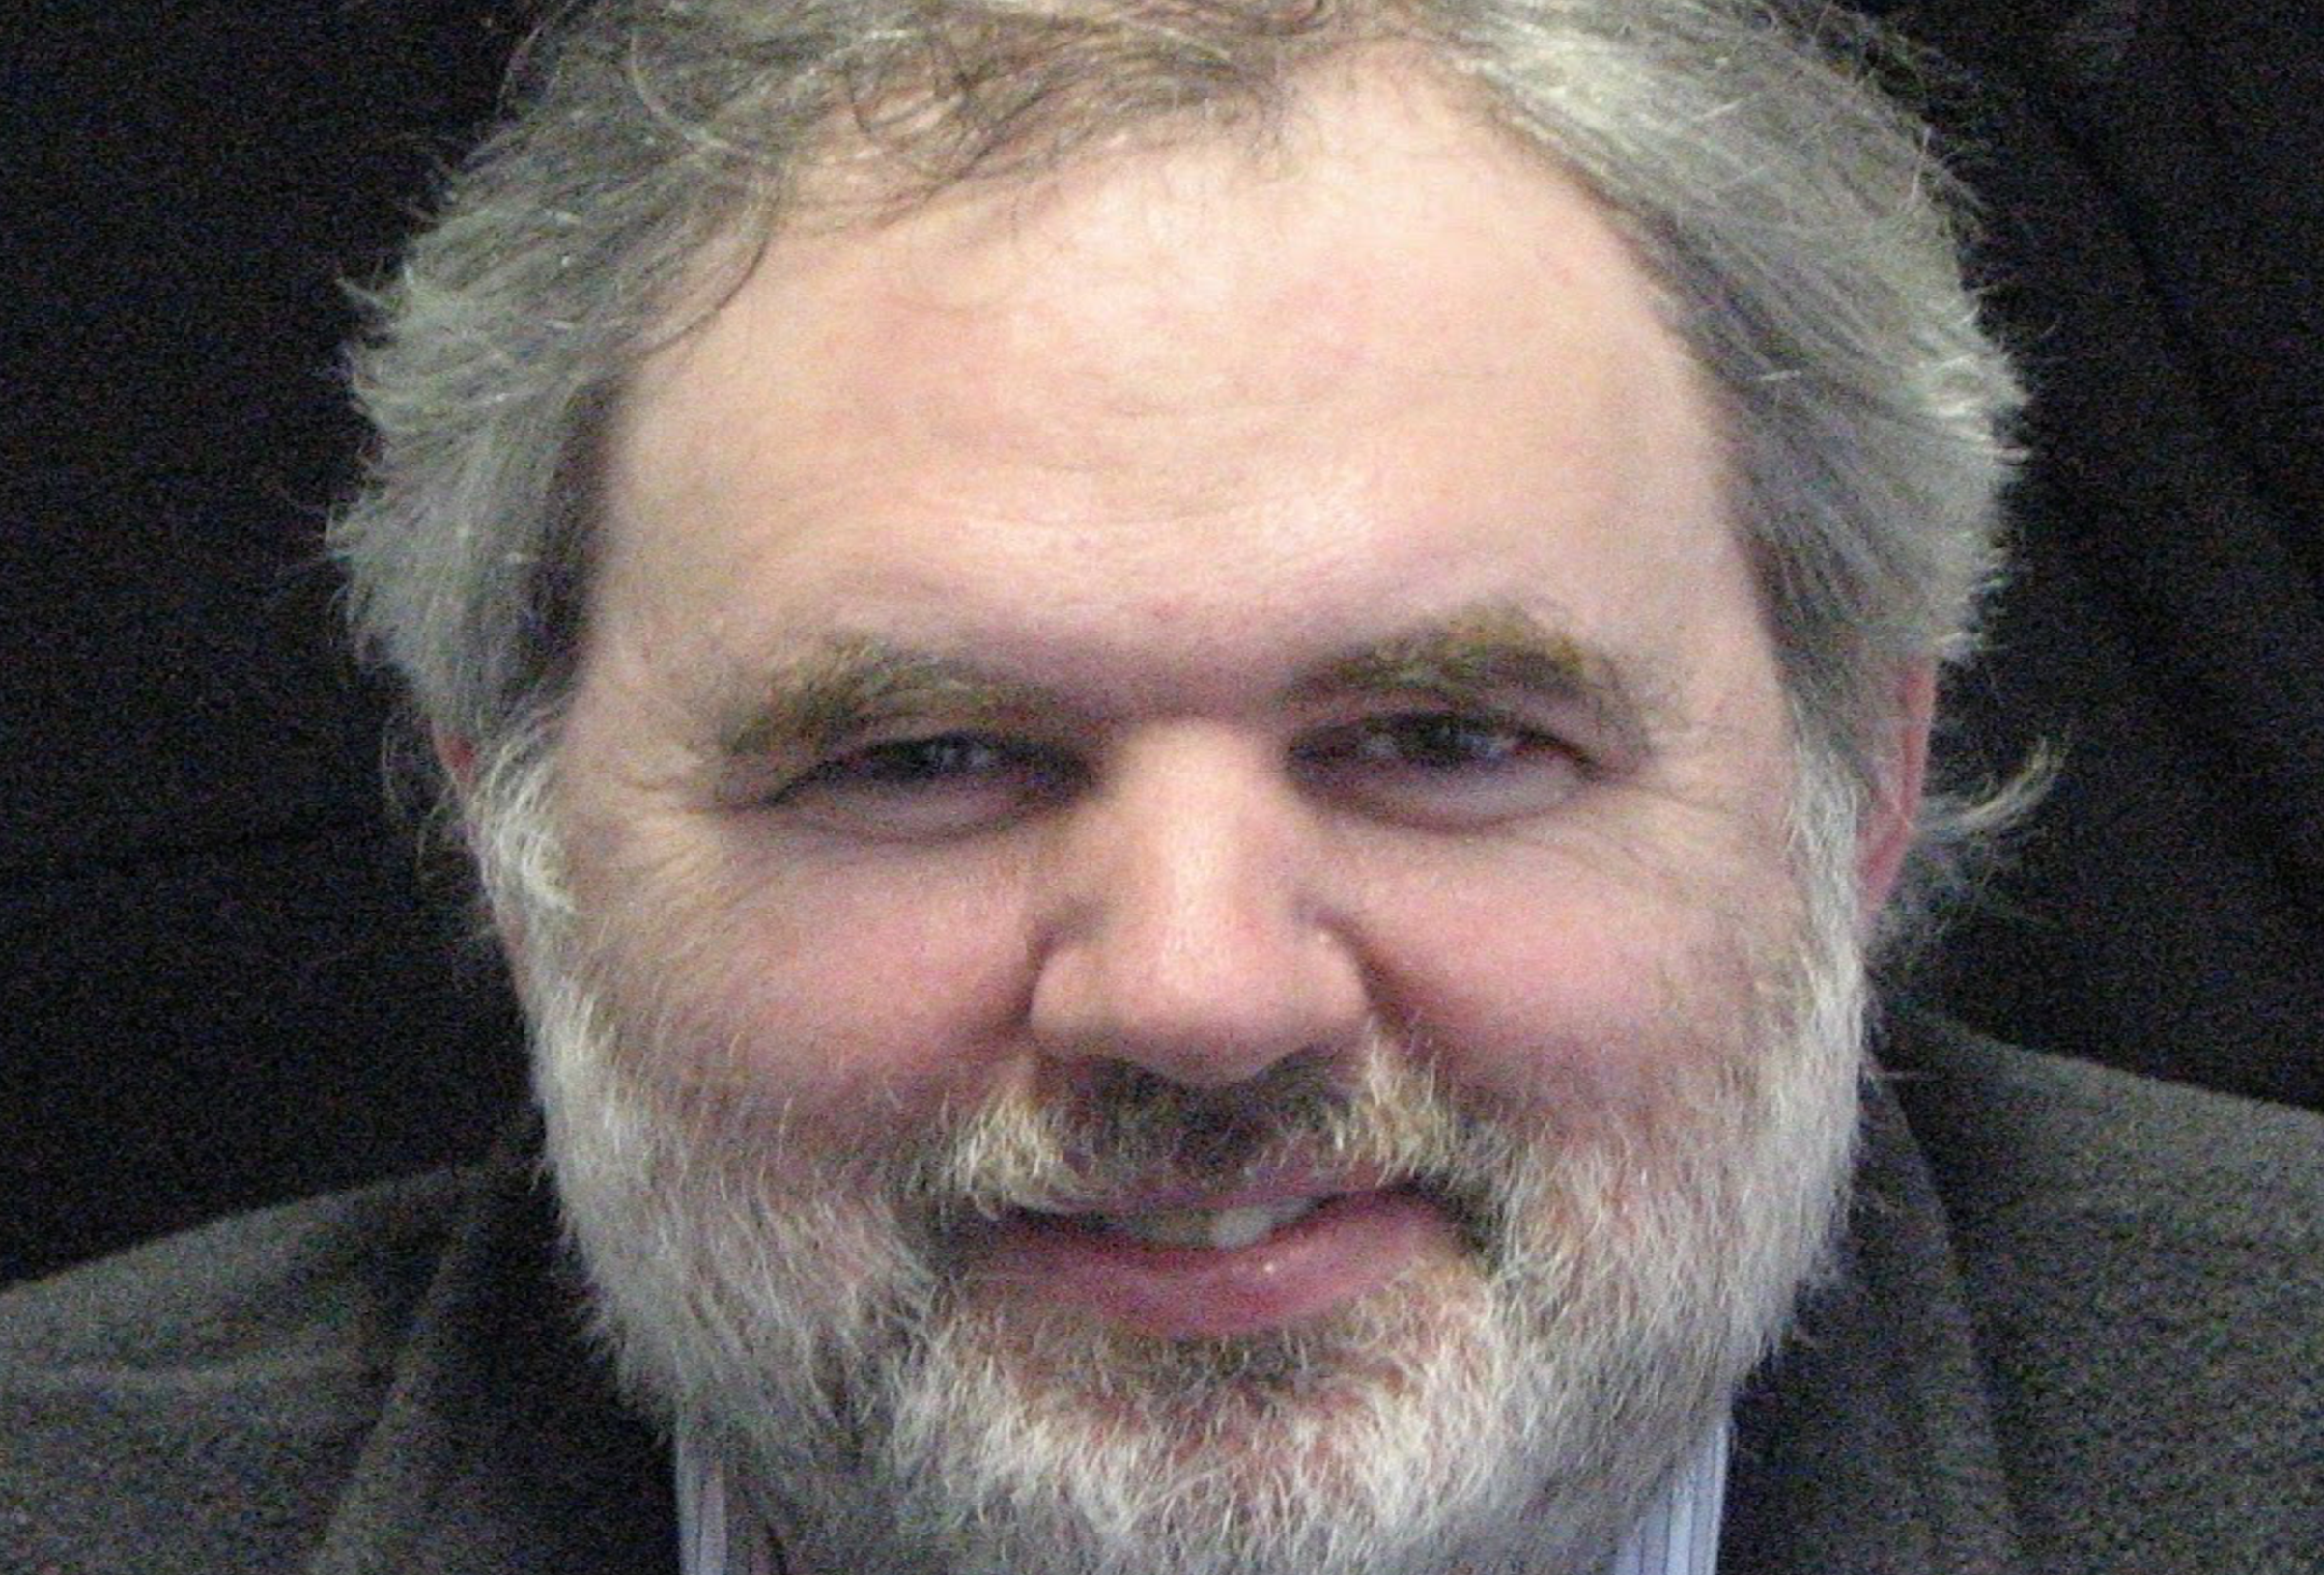
\includegraphics[width=\textwidth]{wlaschin.pdf}
  \\[4pt]
  {\tt https://\textbf{fsharp}forfunandprofit.com/}
\end{frame}

% quote as section
\section["`Well, I Suppose you don't need to know about monads. You only need to use 'Maybe' --~Maybe What? -- 'Maybe' the monad. -- Maybe the monad what? -- Now I think about it. 'Either' might be better... --~Either what?"' \small{(Scott~Wlaschin,~NDC~Conference~2014) [1]}]{Who?}

\begin{frame}{Concept}
  \setcounter{framenumber}{3}
  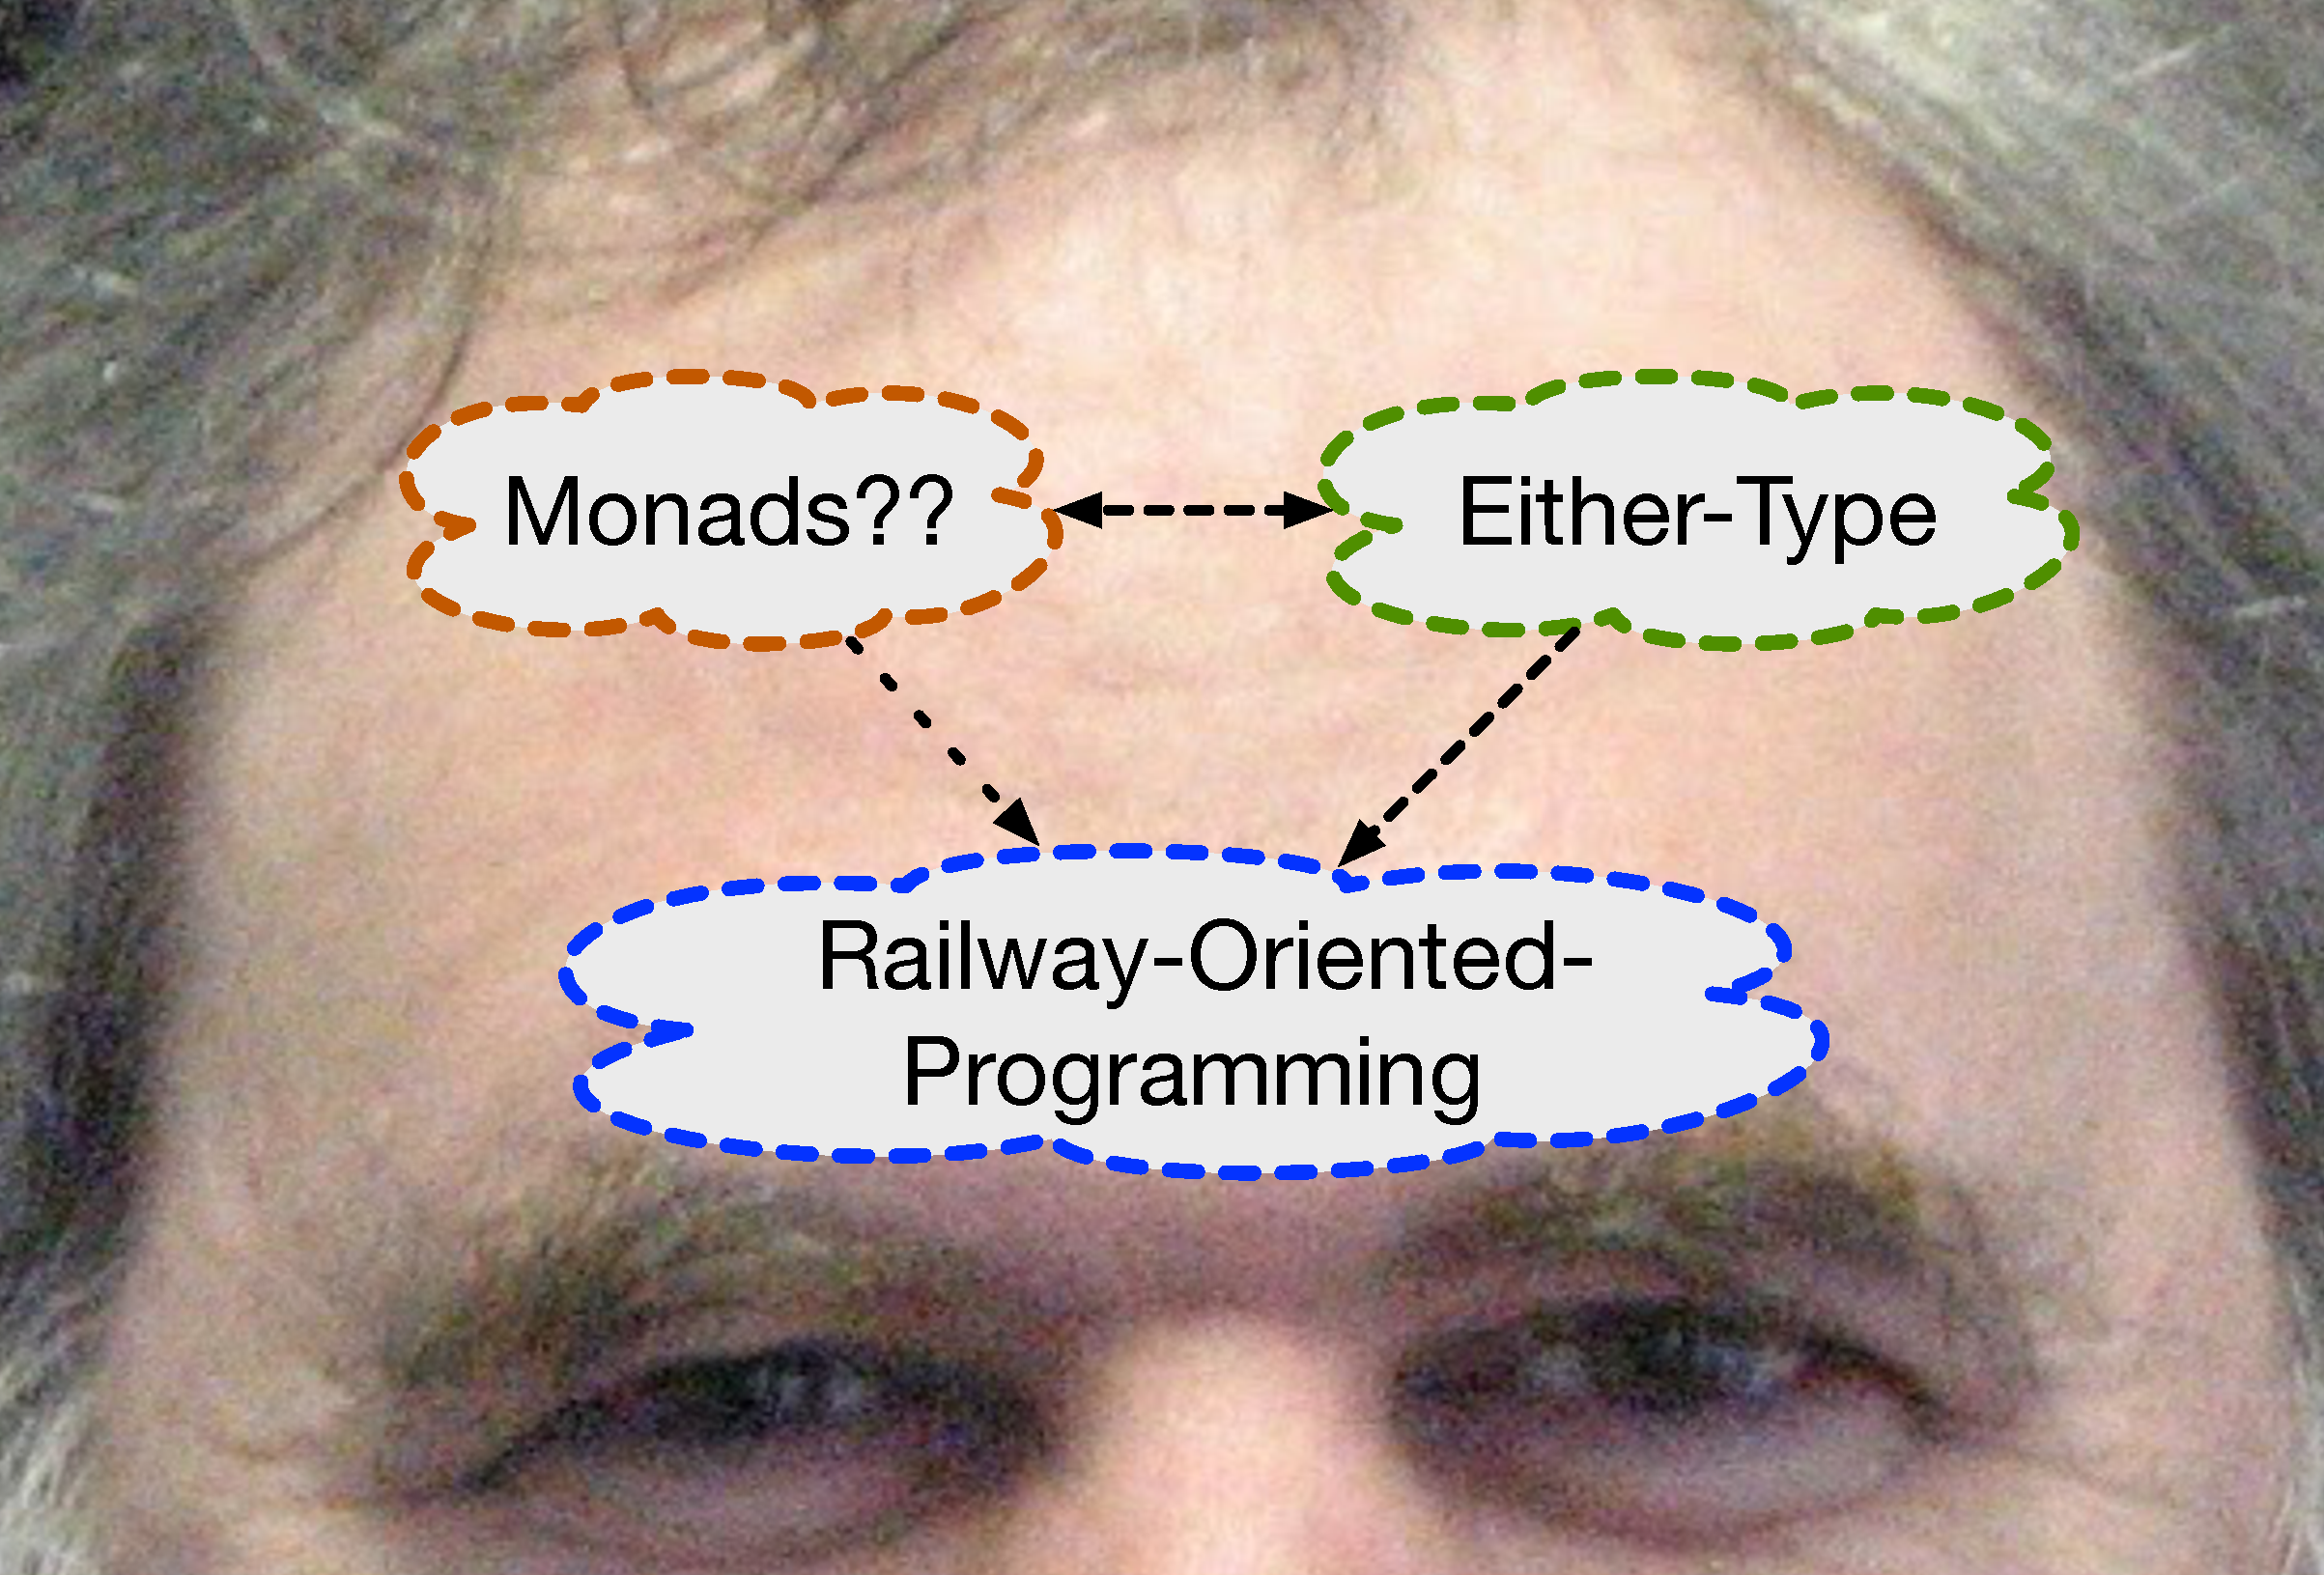
\includegraphics[width=\textwidth]{wlaschin_rop.pdf}
  \\[4pt]
  \texttt{[1] https://vimeo.com/113707214}
\end{frame}

\section{"`Happy-Path"'}
\begin{frame}{Usecase: Update Firstname + Email of User (1/2)}
  \begin{columns}[c]
    \column{.6\textwidth}
    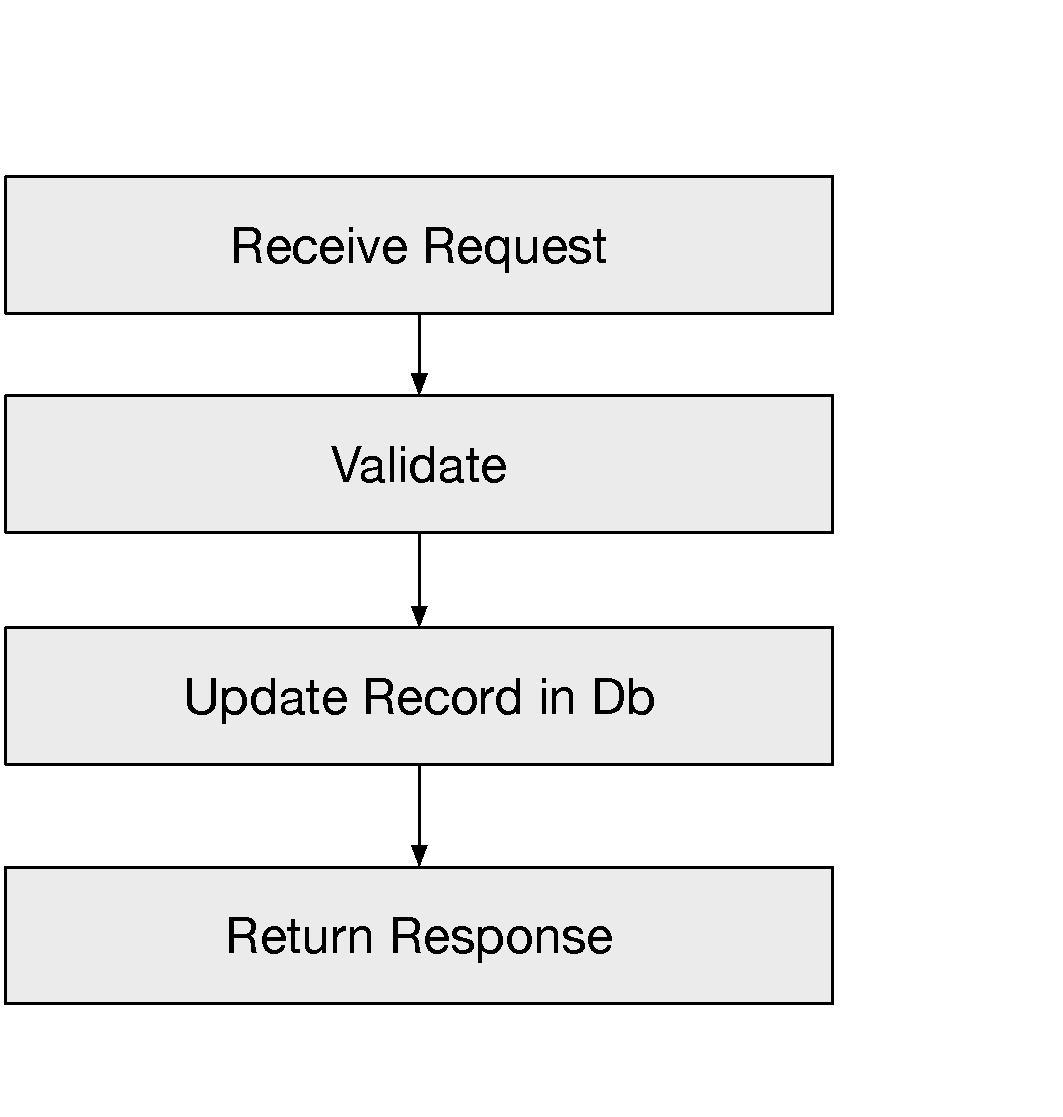
\includegraphics[width=\textwidth]{usecase.pdf}
    \column{.4\textwidth}
    {\tt Request:}
    \\
    \{\\
      "type": ``user",\\
      ``id": ``k48mdsjk",\\
      "firstname": "Max",\\
      ``email": \\~~~~``max@muster.tld"\\
    \}
    \\
    {\tt Response:}
    \\
    \{\\
      "type": ``user",\\
      ``id": ``k48mdsjk",\\
      ``\textit{key}": \textit{value}\\
      ..\\
    \}
  \end{columns}
\end{frame}
\begin{frame}{Usecase happy-path}
  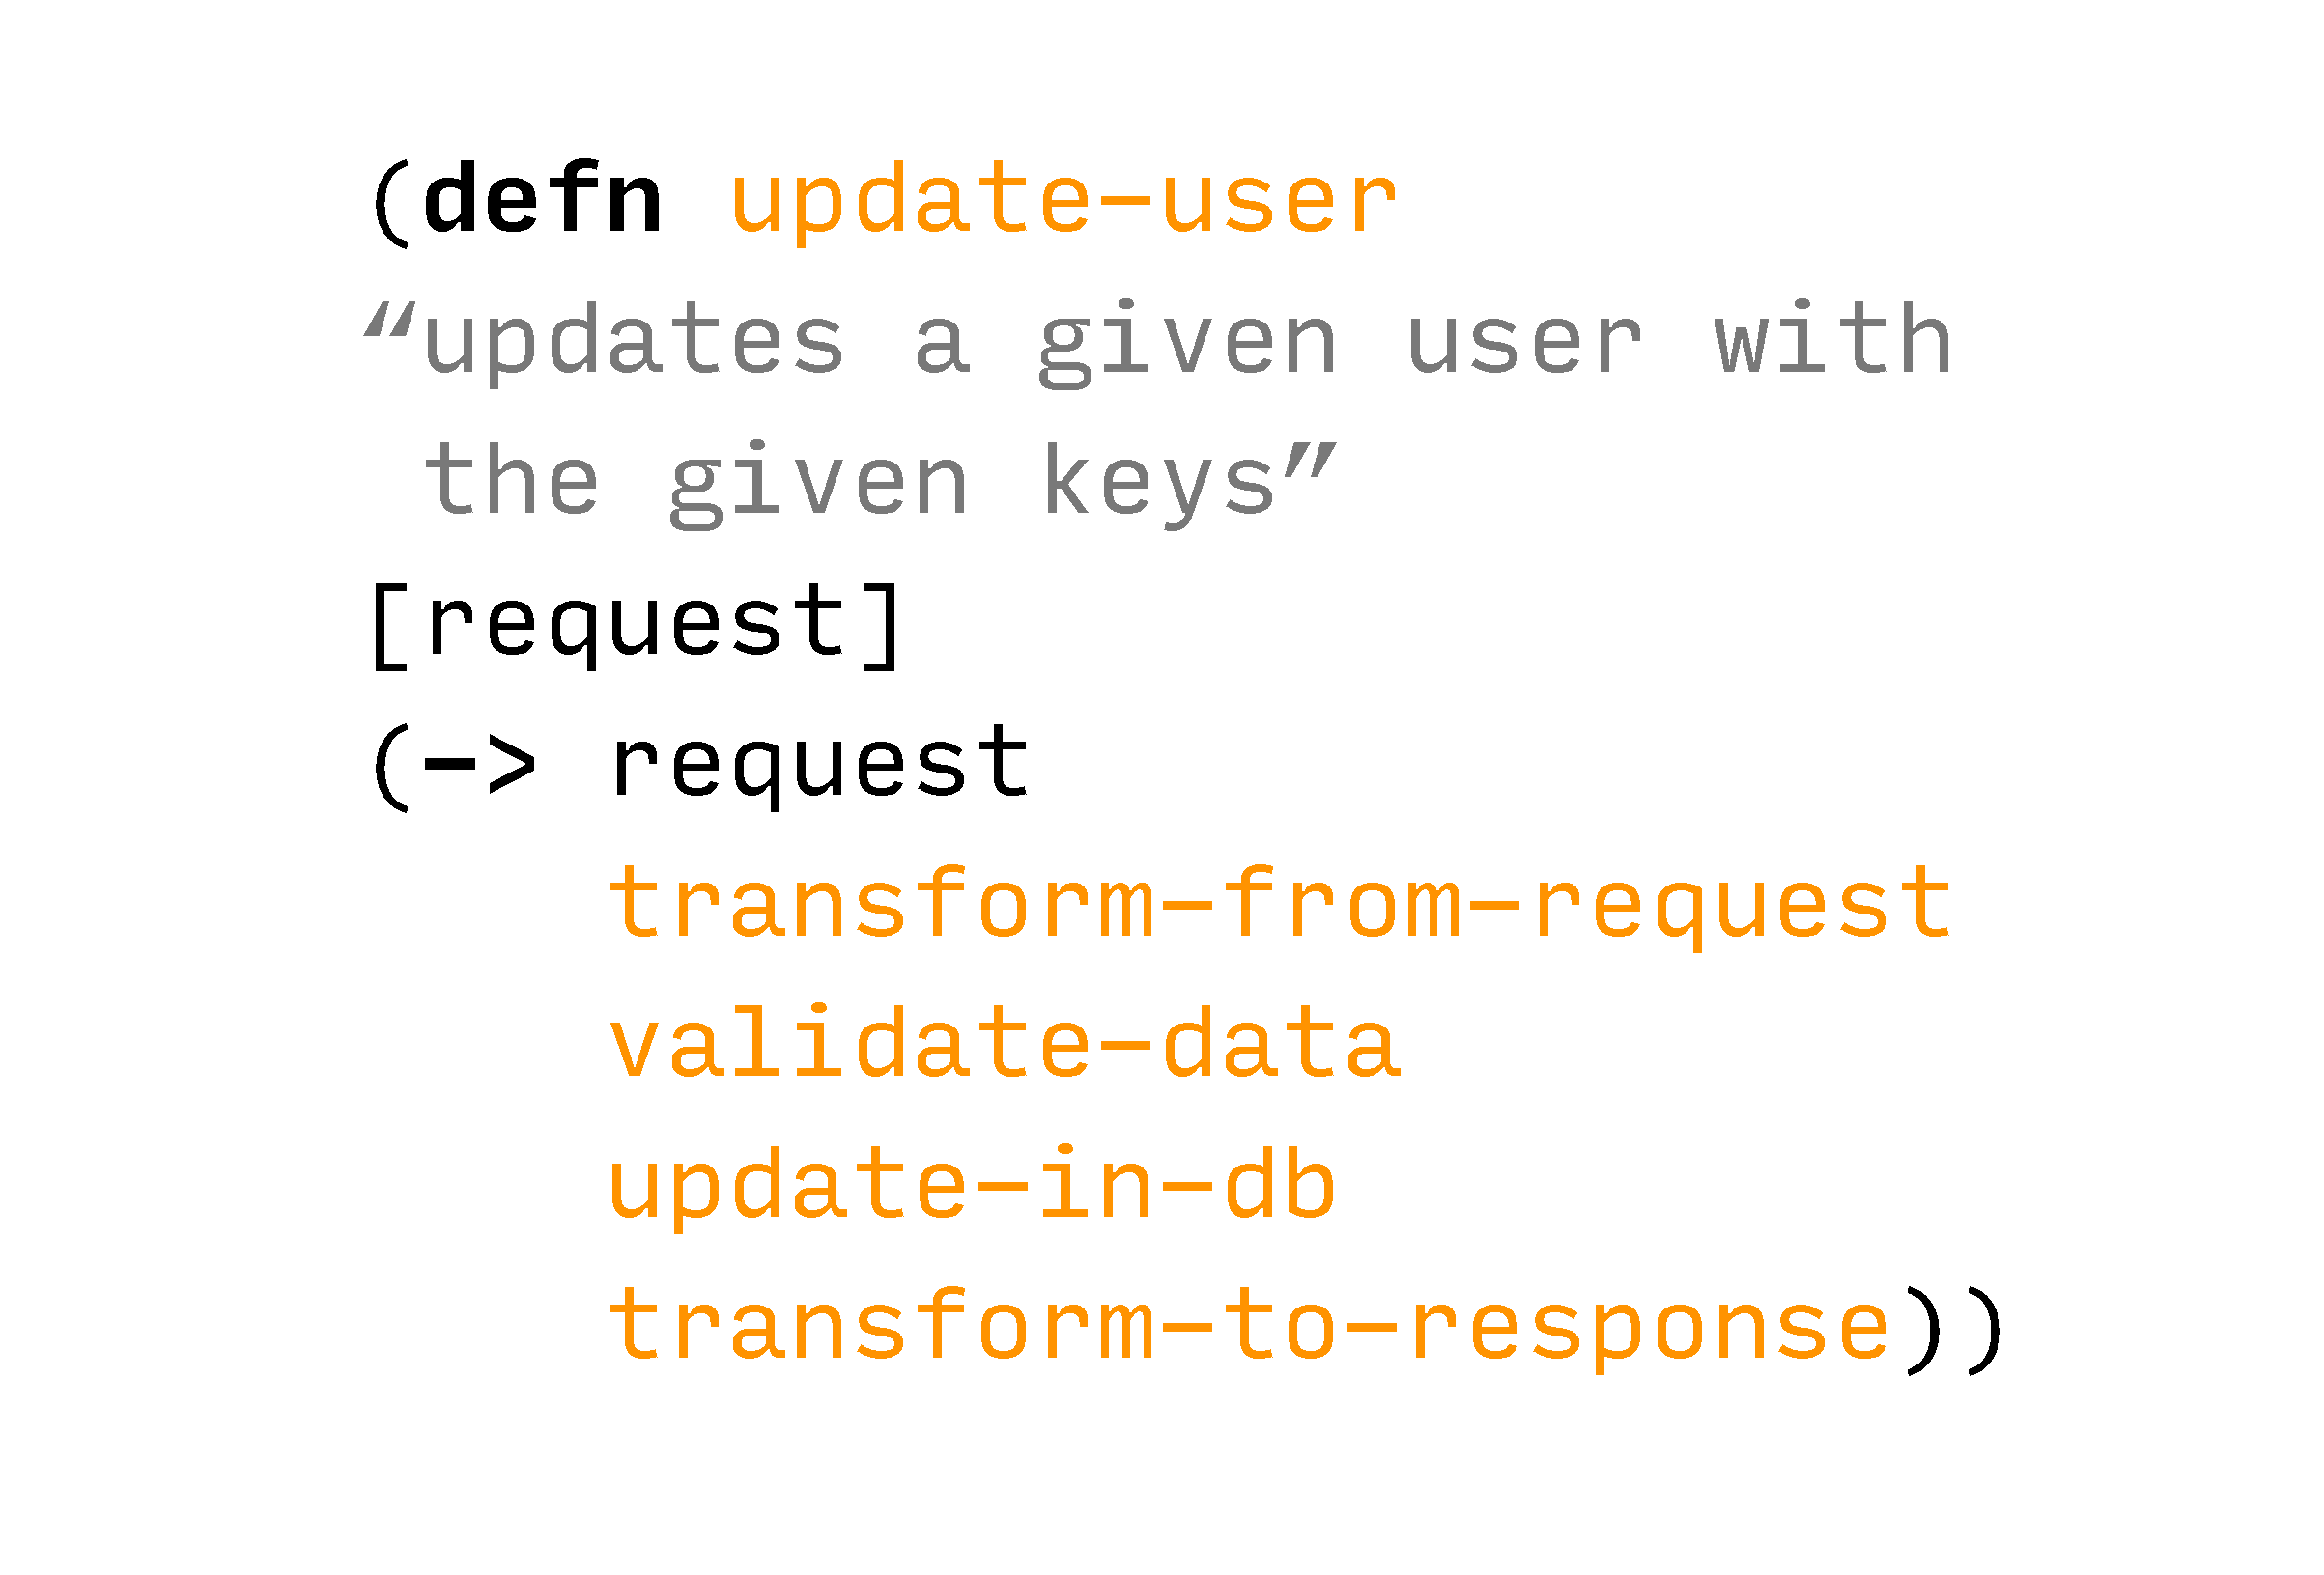
\includegraphics[width=\textwidth]{data_pipe.pdf}
\end{frame}

\section{Error by design}
\begin{frame}{Usecase: Update Firstname + Email of User (2/2)}
  \begin{columns}[c]
    \column{.5\textwidth}
  \textbf{Und sinnvolle Fehler zurückgeben.}
    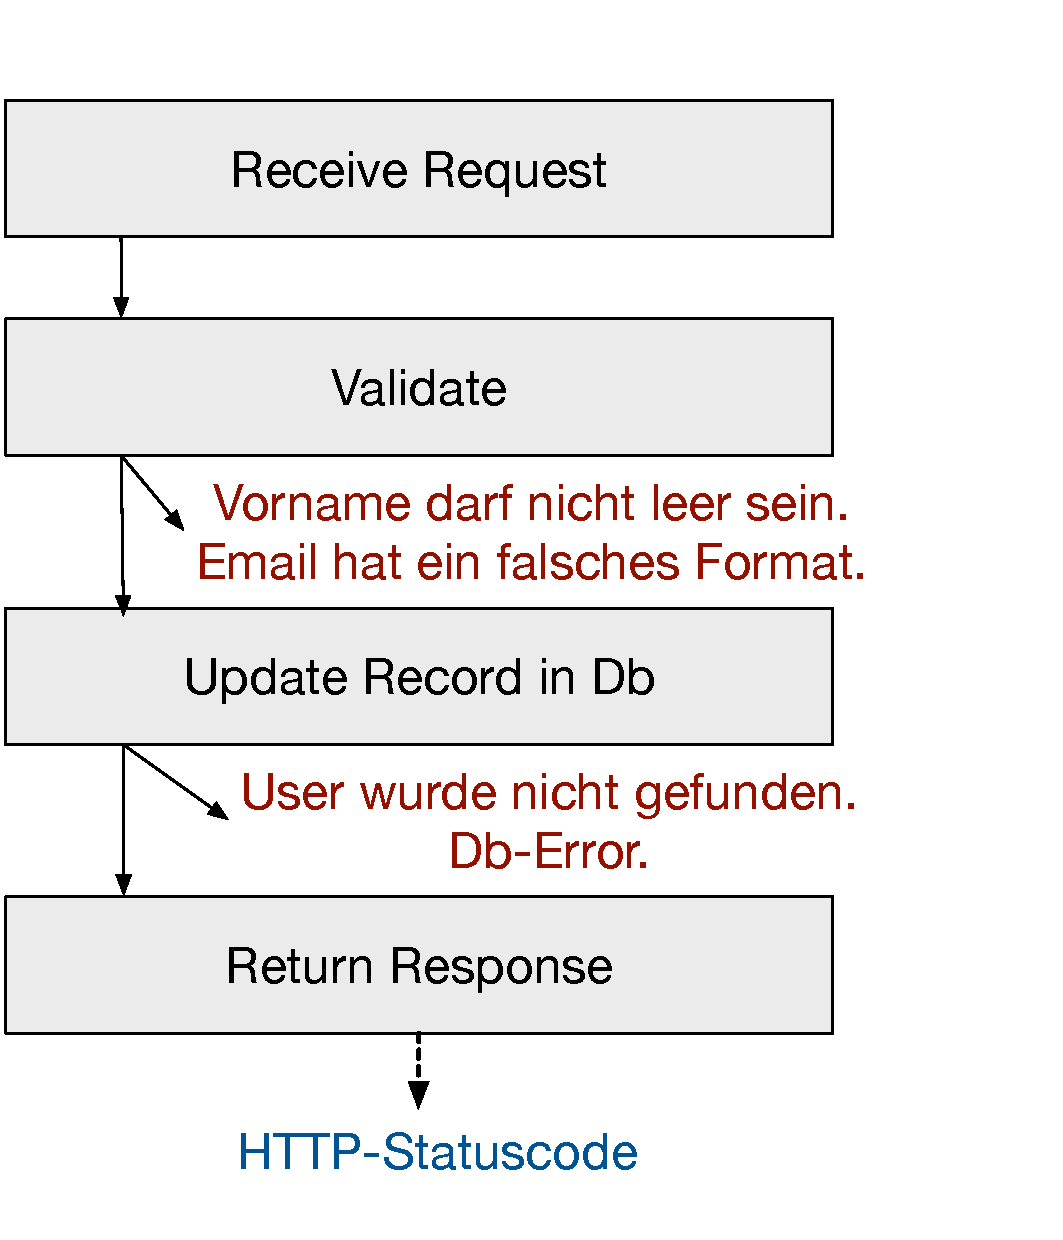
\includegraphics[width=\textwidth]{usecase_error.pdf}
    \column{.5\textwidth}
    {\tt Request:}
    \{\\"type": ``user",\\
      "firstname": `` `` ,\\
      ``email":\\
      ~~~~``max@@@muster.tld"\\
    \}
    \\
    {\tt Response:}
    \{\\
      "result": \{\\
      ~~``success": \{\\~~~~"type": ``user",\\
      ~~~~``id": ``k48mdsjk",\\
      ~~~~``\textit{key}": \textit{value}\\
      ~~~~..\\
      ~~\}\\
    \}
    \\
    \texttt{Header: 200 OK | ..}
  \end{columns}
\end{frame}
\begin{frame}{Usecase mit Error-Handling}
  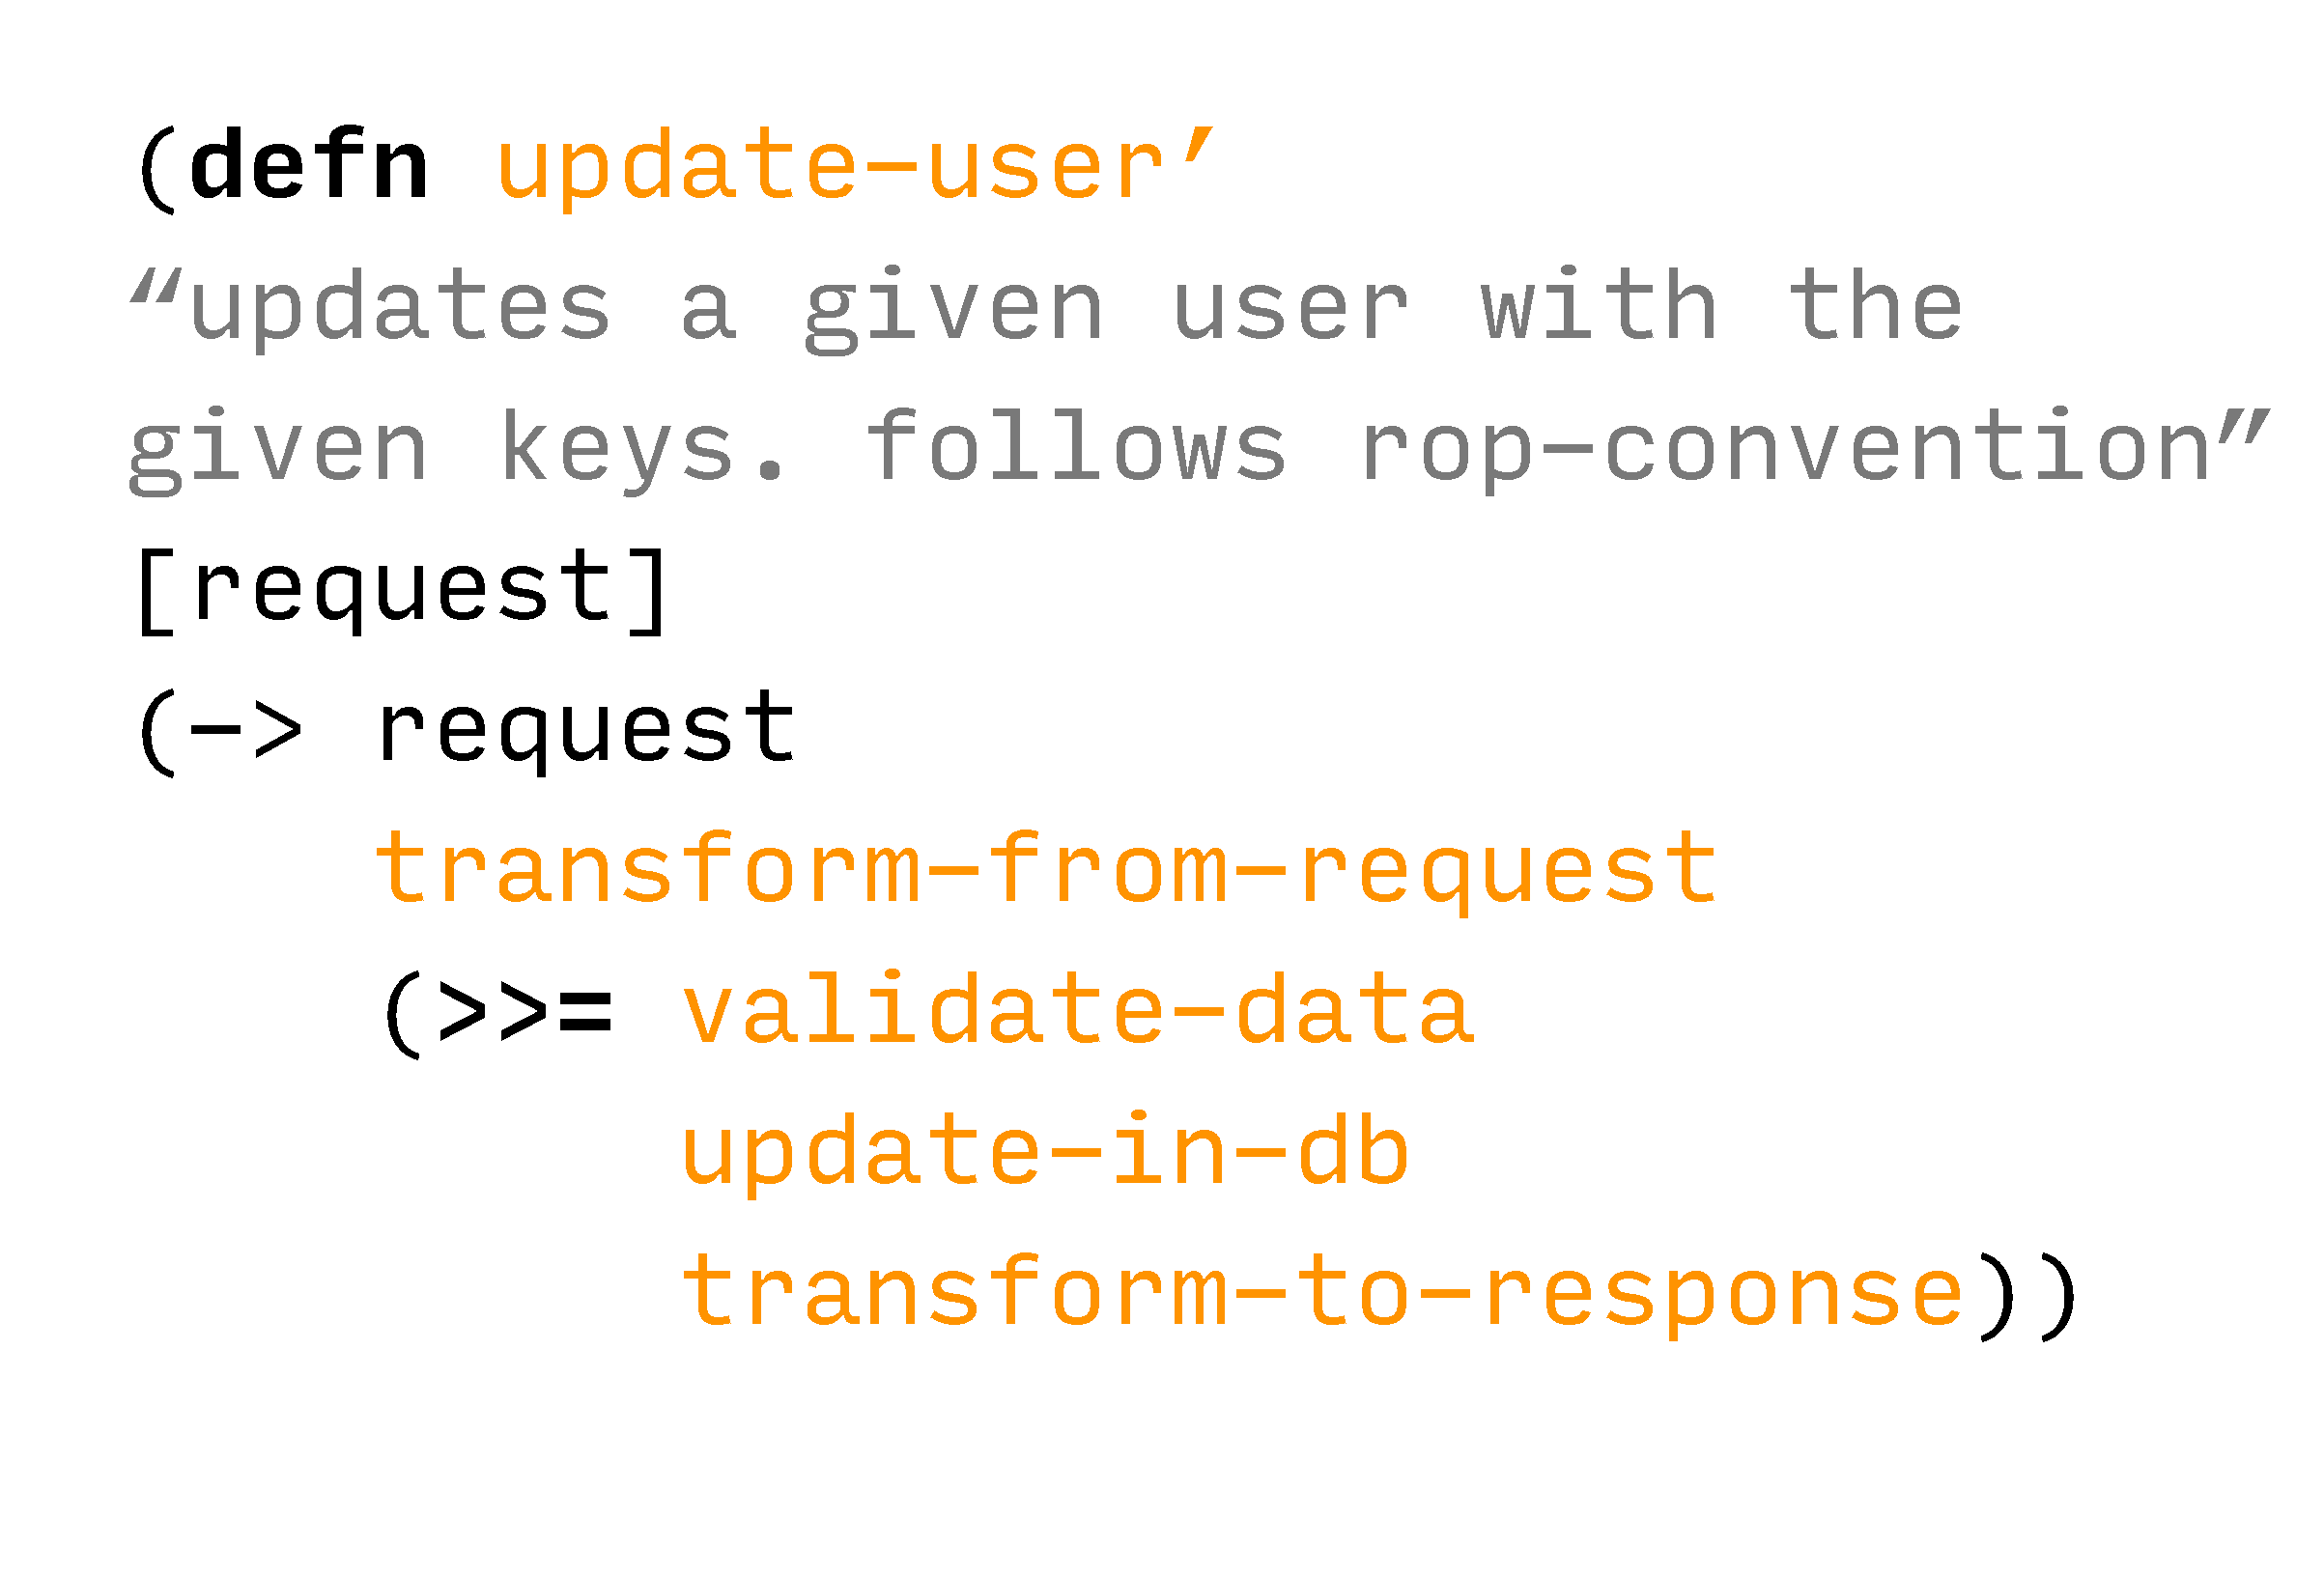
\includegraphics[width=\textwidth]{data_pipe_error.pdf}
\end{frame}

\section{"`Railway-Oriented-Programming"'}
\begin{frame}{Grundlegende Schienenteile}
  % \begin{columns}[c]
  % \column{.5\textwidth}
  % \begin{itemize}
  %   \item succeed-fail
  %   \item switch-function
  %   \item bind
  %   \item pipe-bind
  %   \item switch-compose
  %   \item core, core.match
  %   \item clojure seq-abstraction
  %   \item rest-parameters, map, apply
  % \end{itemize}
  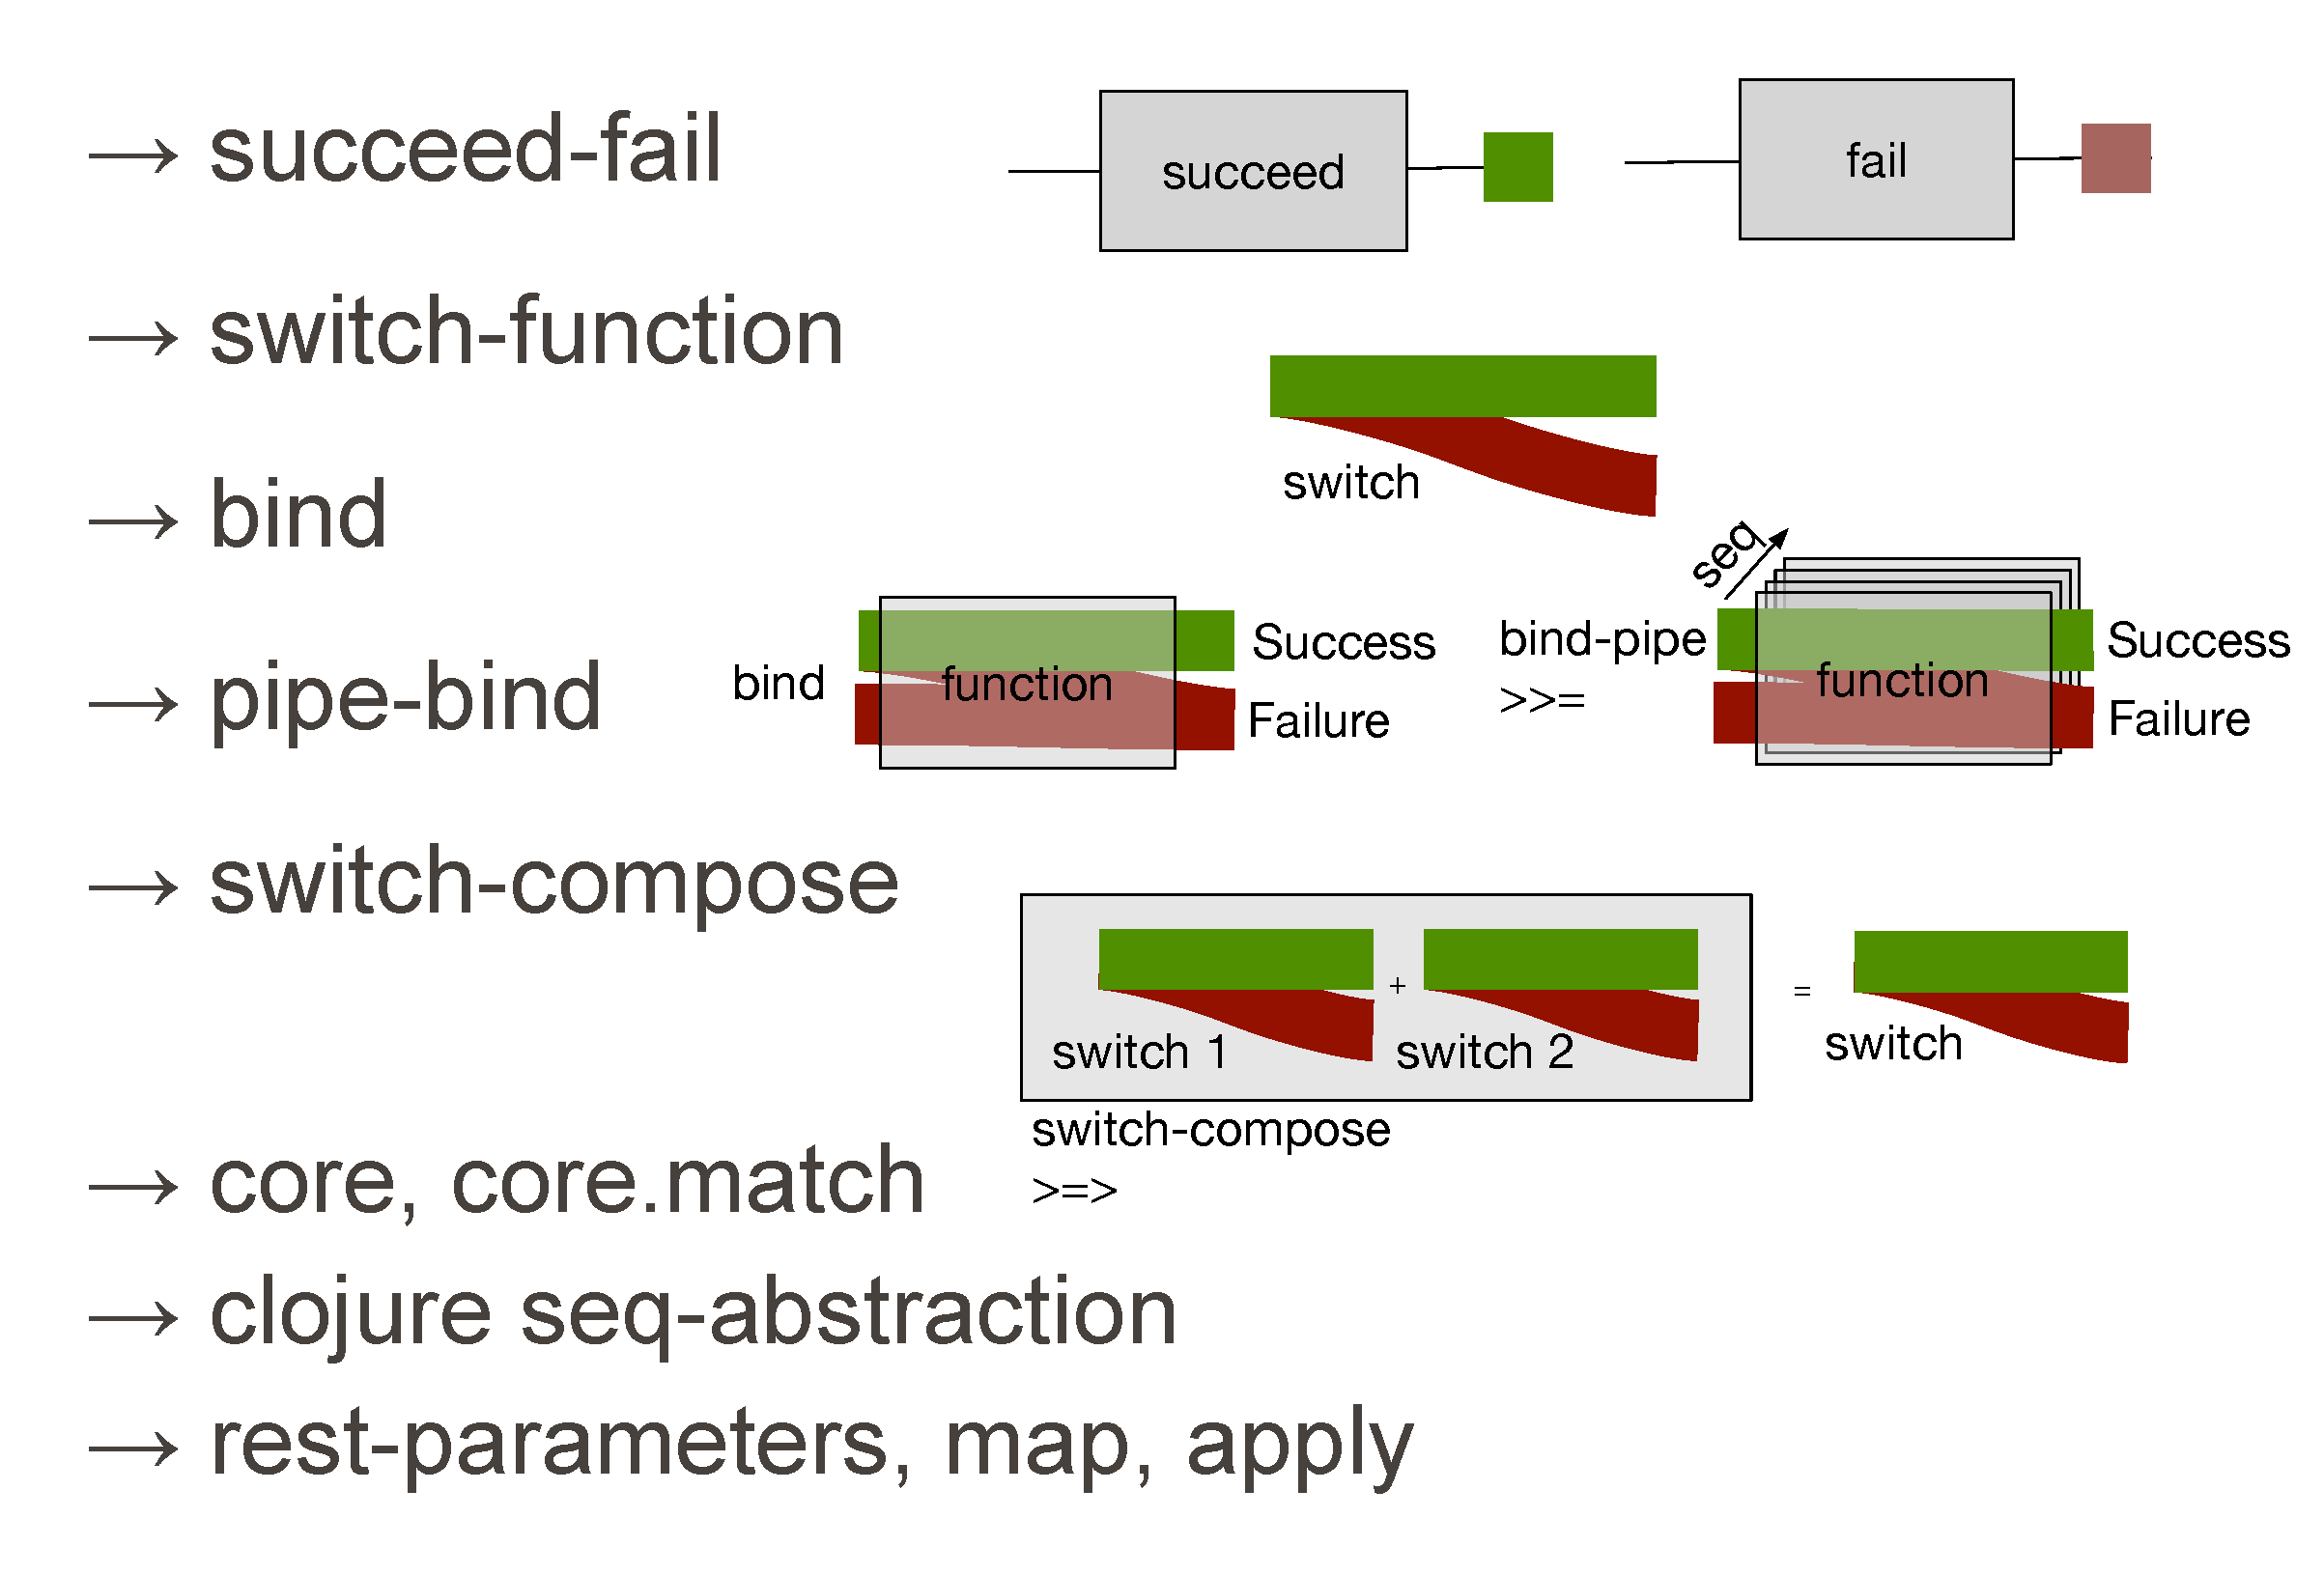
\includegraphics[width=\textwidth]{rails_overview.pdf}
  % \column{.5\textwidth}
  % \includegraphics[width=\textwidth]{parallel.pdf}
  % \end{columns}
\end{frame}
\begin{frame}{succeed \& fail}
%   \begin{itemize}
%     \item \texttt{(succeed 'Hello Clojure!')}
% \item \texttt{(fail 'Oh no!')}
% \end{itemize}
  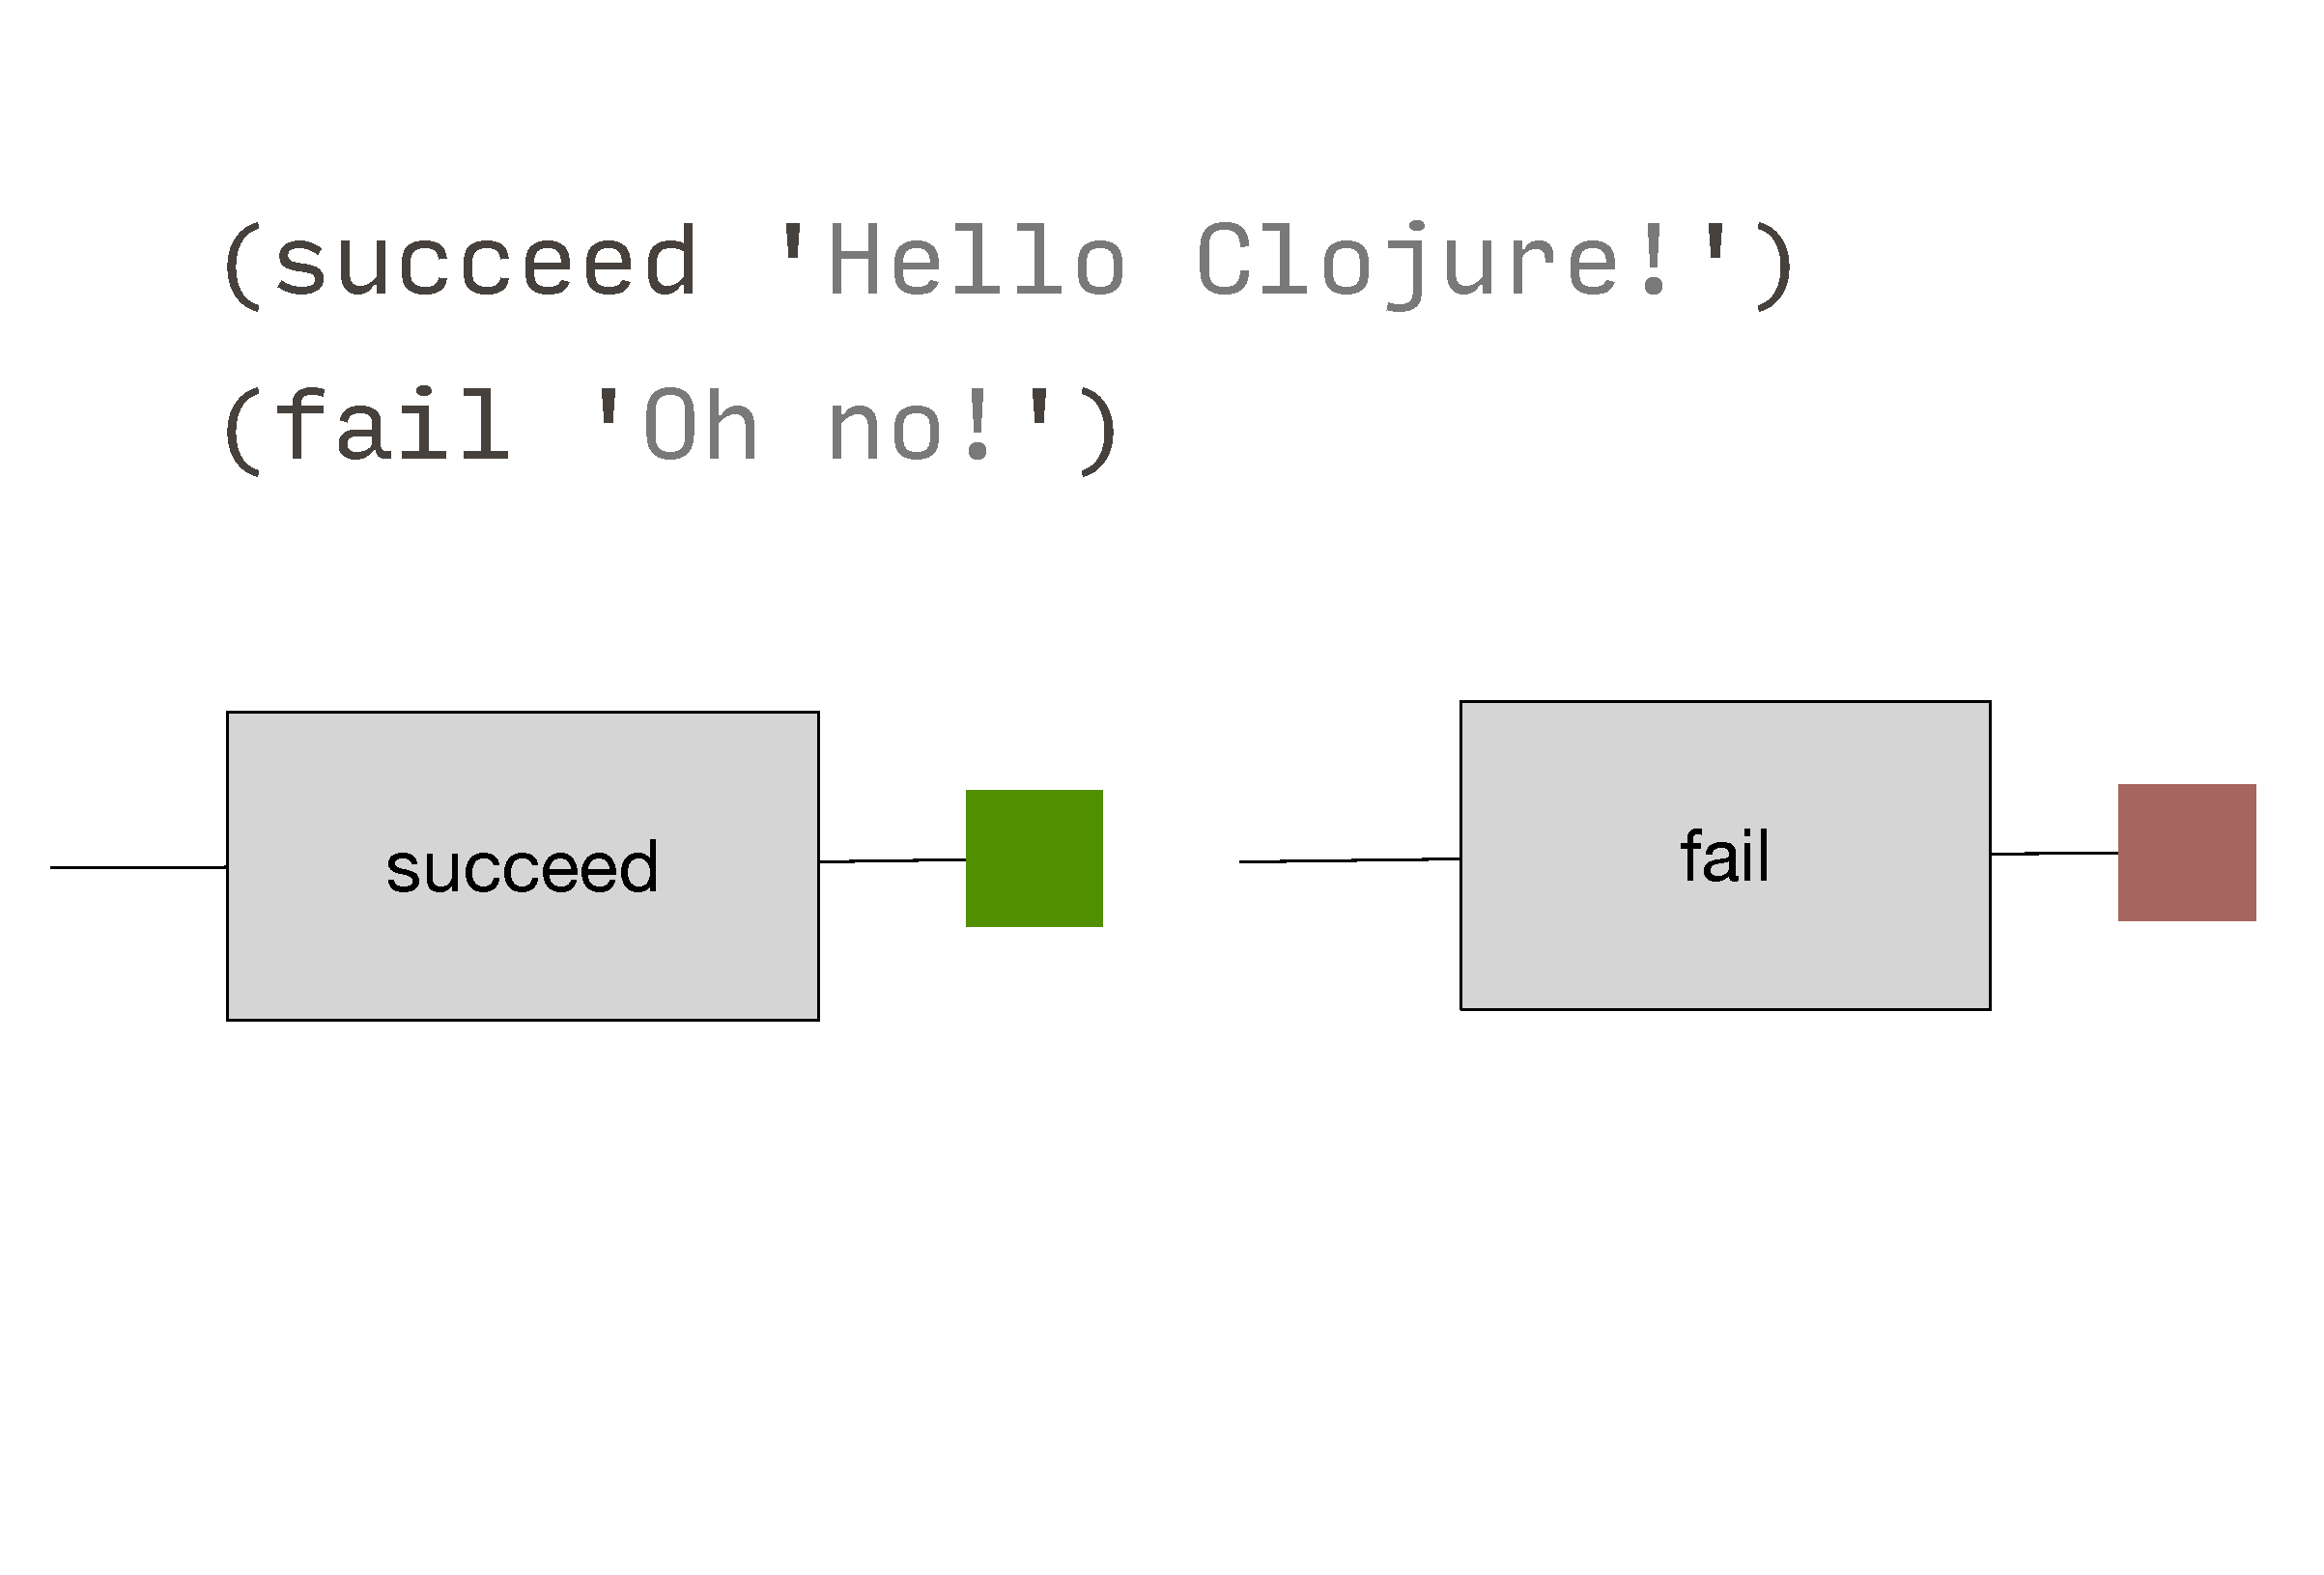
\includegraphics[width=\textwidth]{succeed_fail.pdf}
\end{frame}
\begin{frame}{switch-function}
  % \begin{itemize}
  %   \item \texttt{((switch +) 2 2)}
  % \end{itemize}
  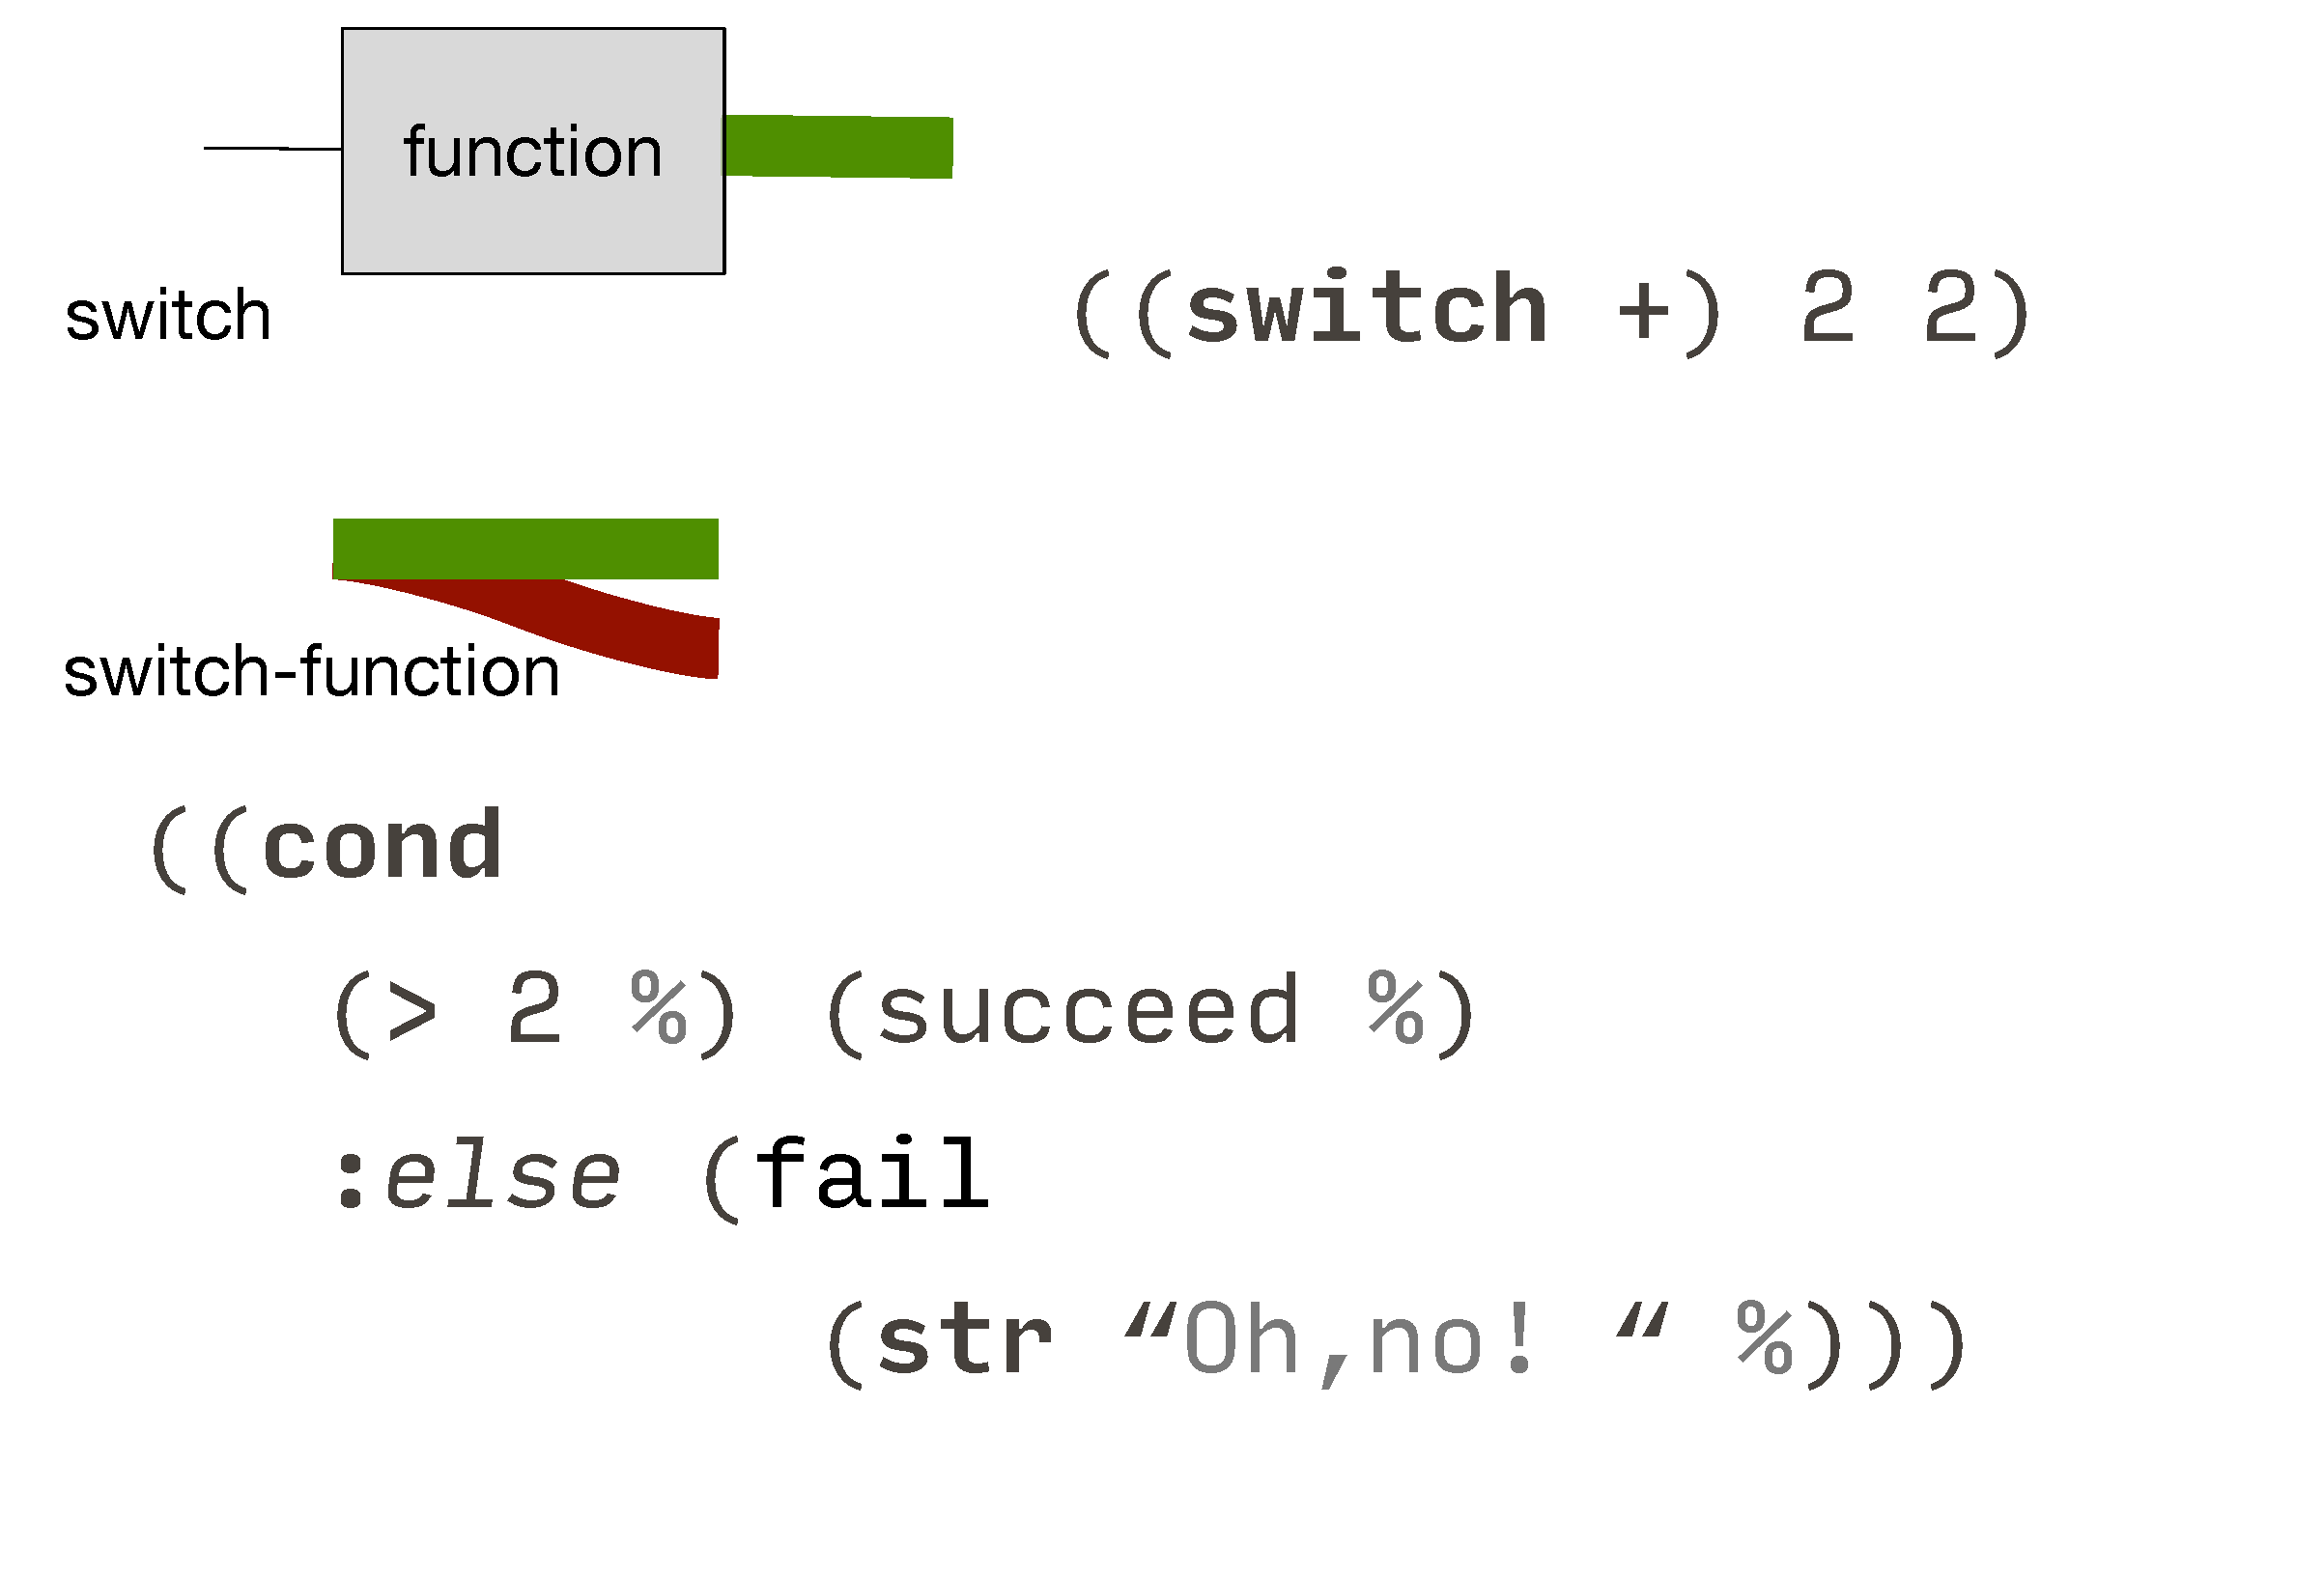
\includegraphics[width=\textwidth]{switch.pdf}
\end{frame}
\begin{frame}{bind}
  % \begin{itemize}
  %   \item \texttt{((bind \#(succeed \%)) (succeed "42"))}
  %   \item \texttt{((>>= \#(succeed \%) \#(fail (str "Fehler: " \%))) \\(succeed "42"))}
  % \end{itemize}
  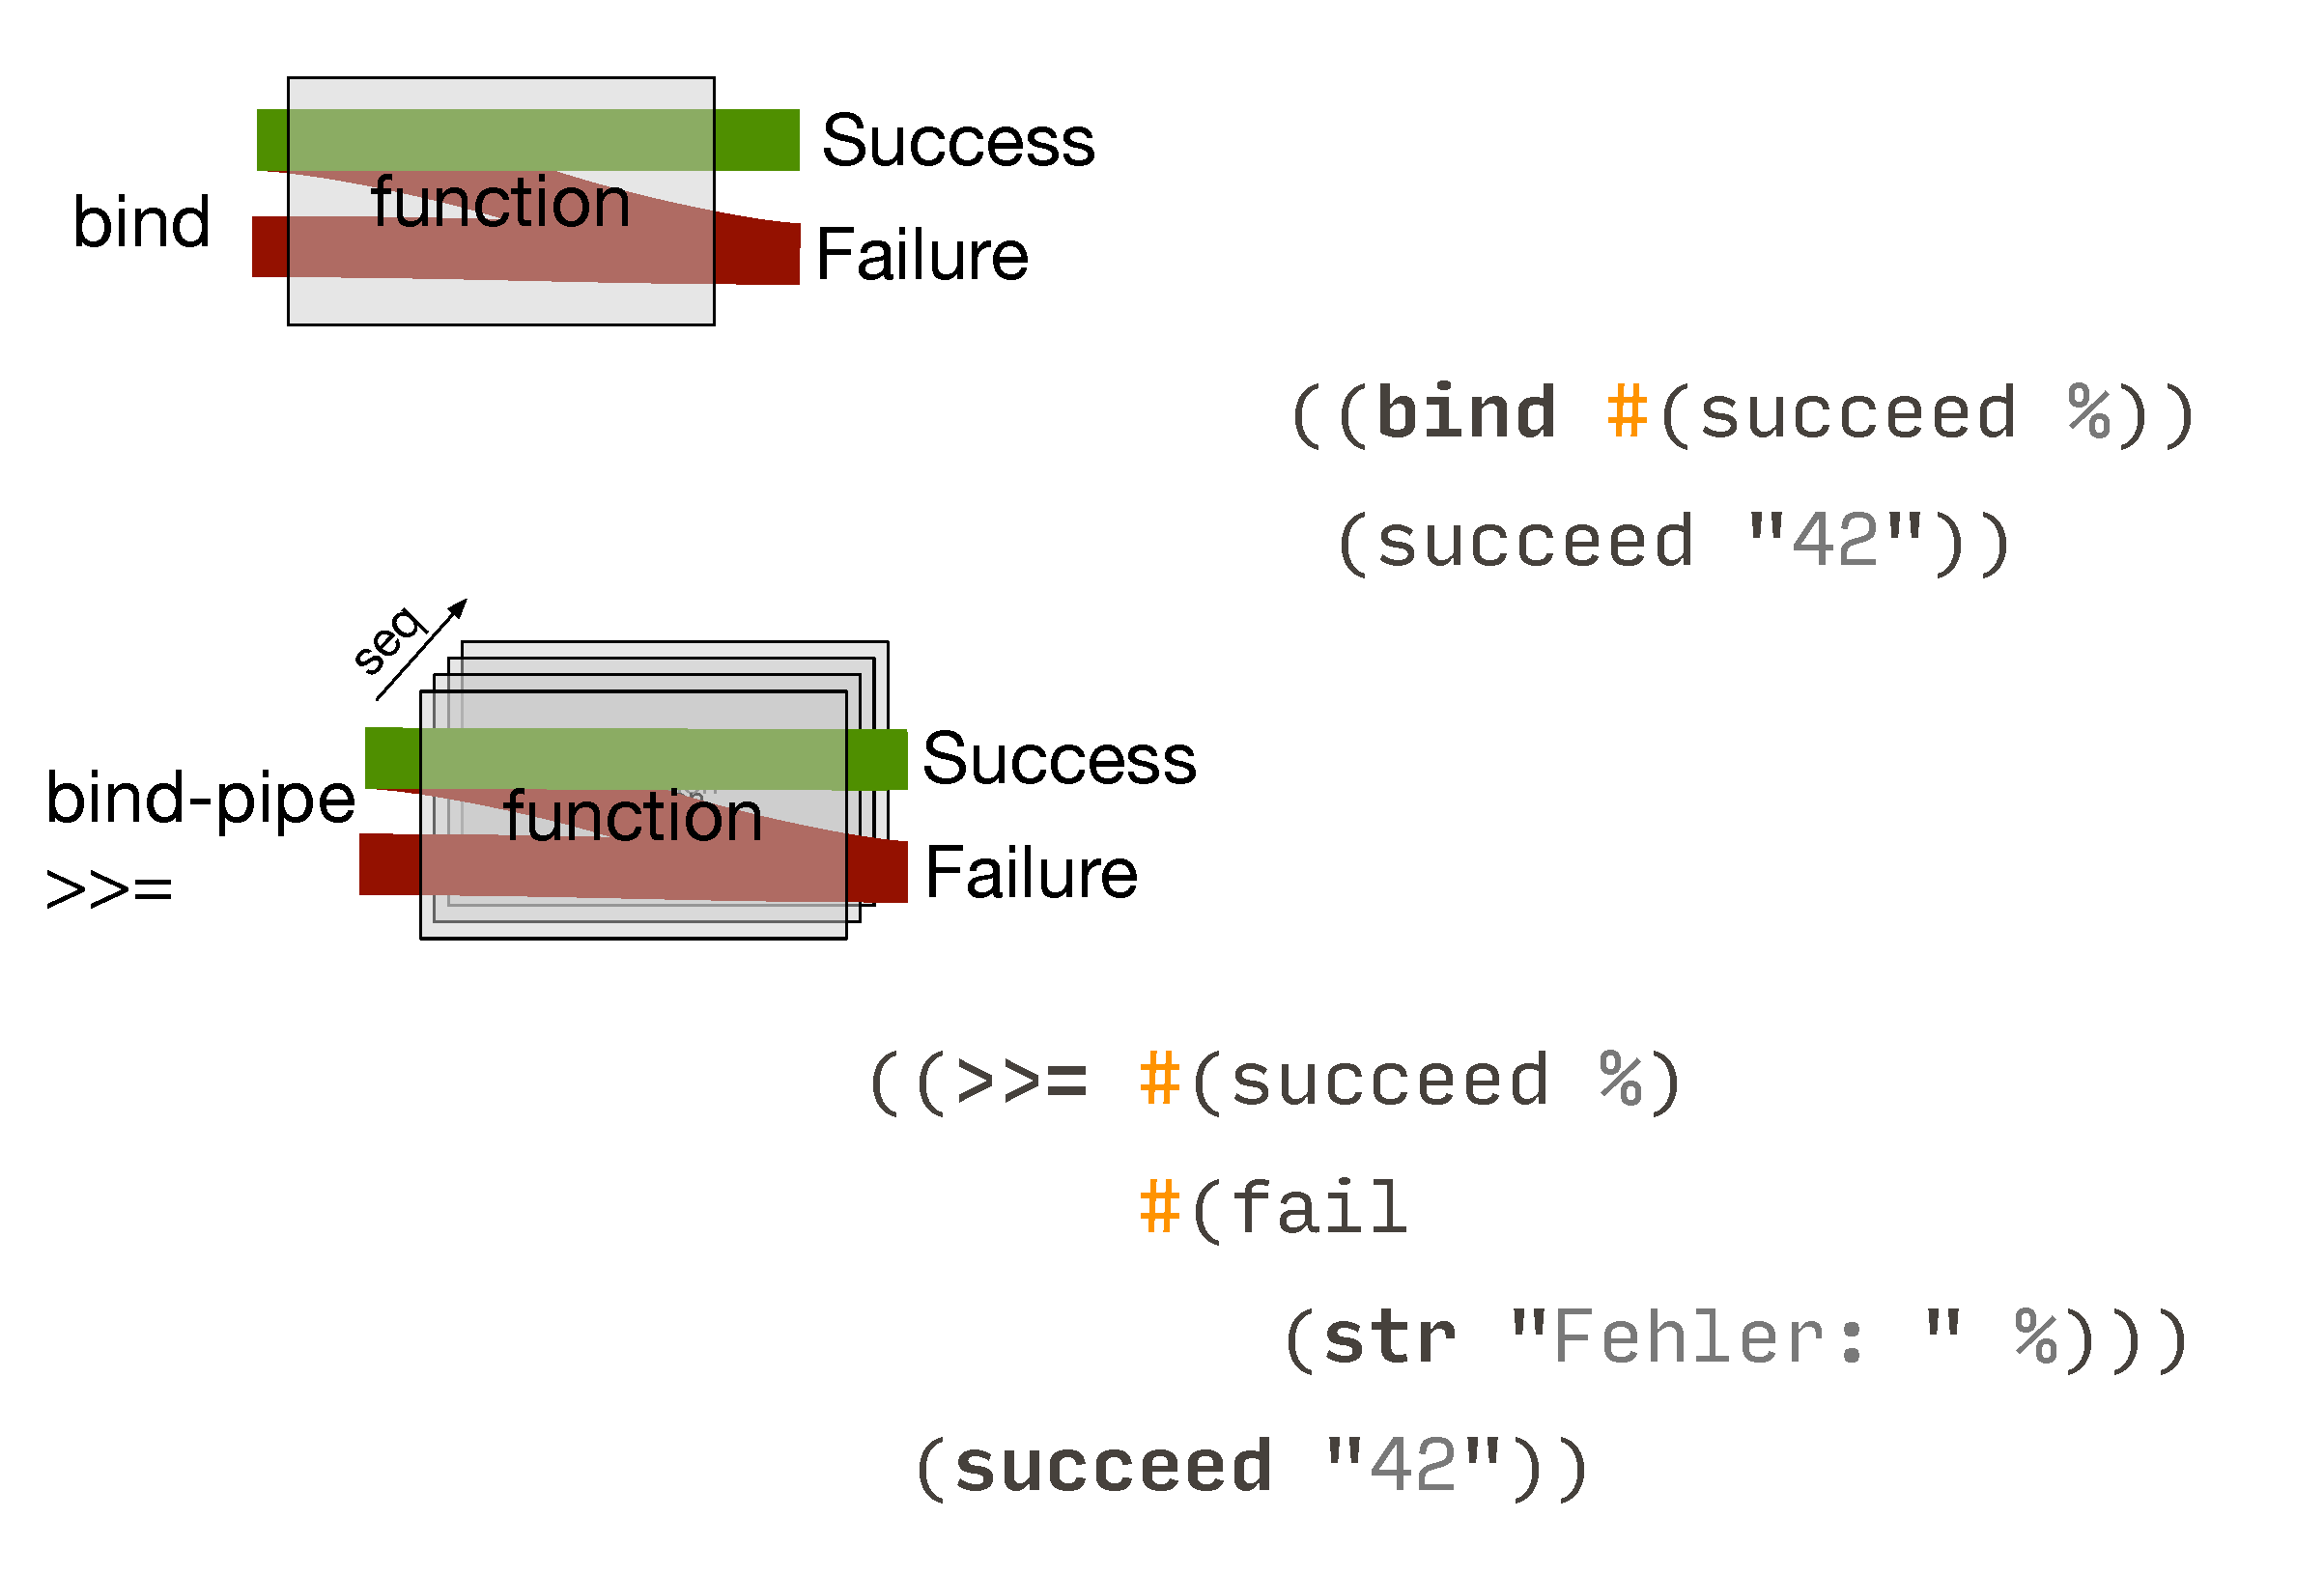
\includegraphics[width=\textwidth]{bind.pdf}
\end{frame}
\begin{frame}{compose}
  % \begin{itemize}
  %   \item \texttt{((>=> ((switch +) 2 2)((switch *) 2))\\ (succeed "42"))}
  % \end{itemize}
  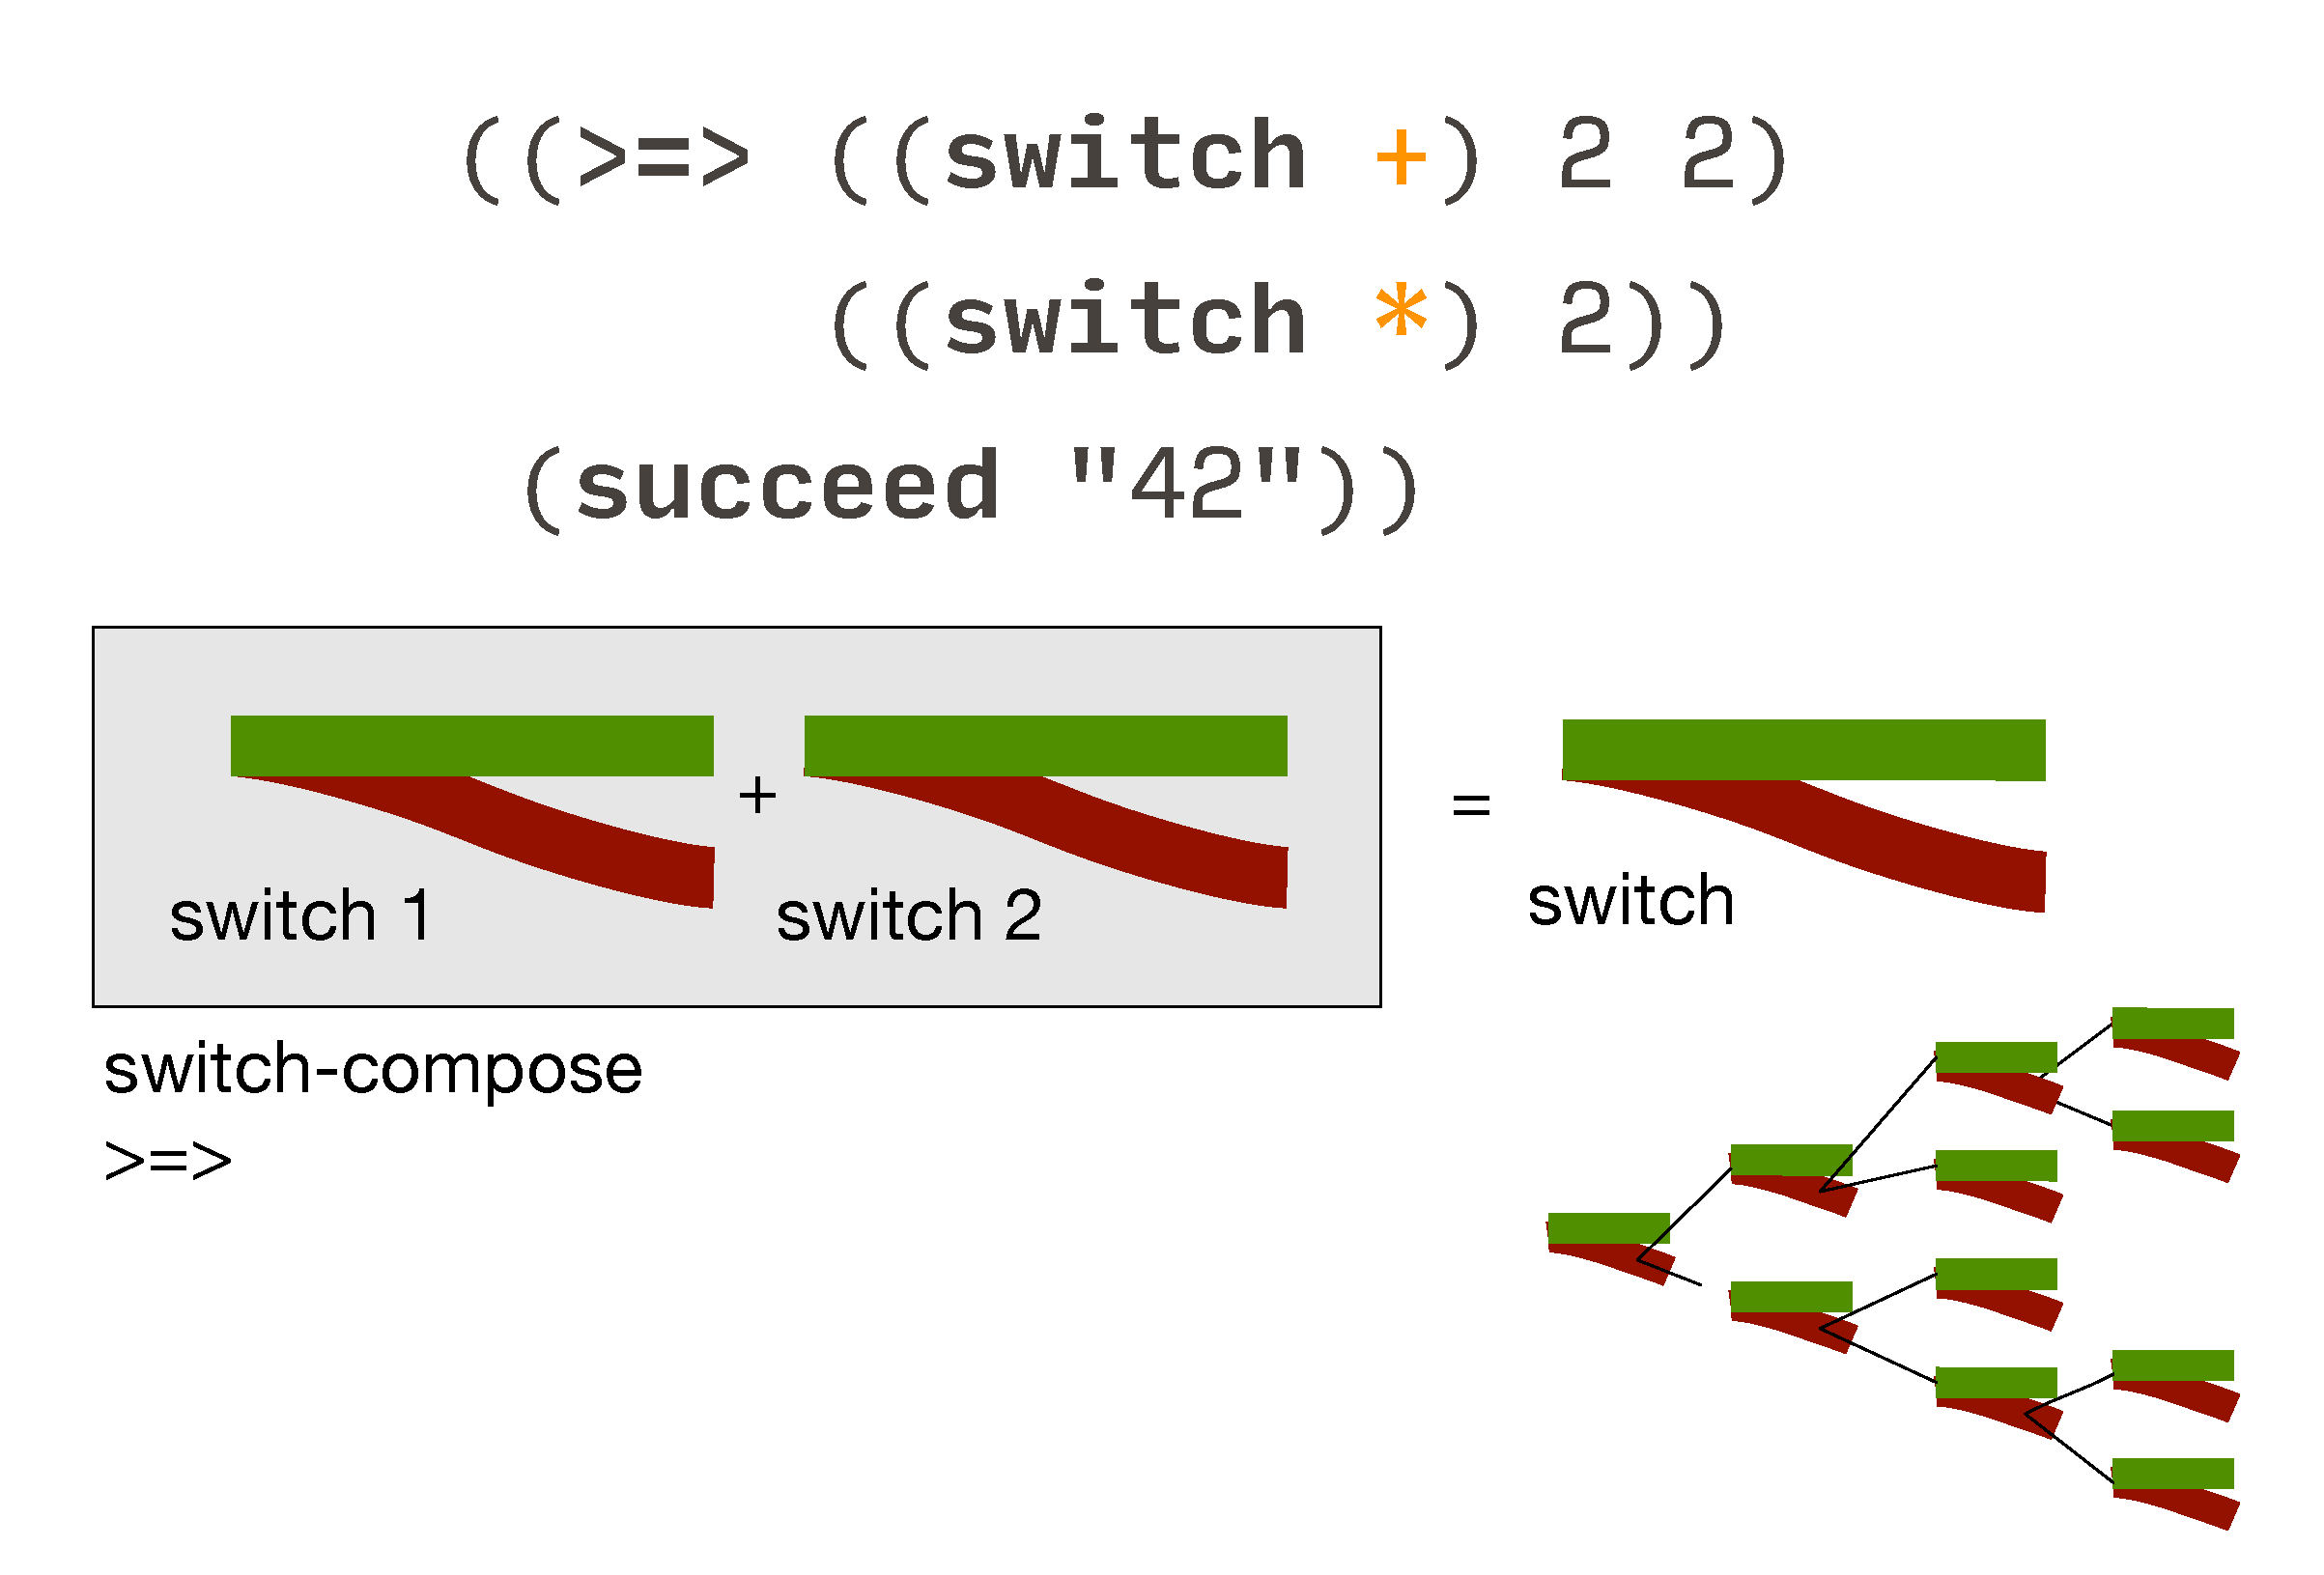
\includegraphics[width=\textwidth]{compose.pdf}
\end{frame}
% \begin{frame}{User-Validation mit ROP}
%   detail
% \end{frame}

% \note[itemize]{%
%     \item 
% }

\section{Ausblick}
% \begin{frame}{Äpfel \& Birnen}
%   unterschied compose und bind
%   \\
%   als grafiken
% \end{frame}
\begin{frame}{Weitere Schienenteile}
  \begin{itemize}
    \item try/catch
    \item log
    \item tee
    \item map-parallel
    \item ..beliebig als Basis nutzbar
  \end{itemize}
\end{frame}
\begin{frame}{Fazit}
  \begin{itemize}
    \item kann am Anfang im Vergleich sehr kompliziert sein
    \item bei konsistenter Anwendung wirklich hilfreich
    \item Data-Flow mit Step pro Usecase wird angestrebt
    \item leicht erweiter- und wartbar
  \end{itemize}
\end{frame}

\begin{frame}[noframenumbering,plain]{Fin}
  Danke für die Aufmerksamkeit. -- Fragen?
\end{frame}
\begin{frame}[noframenumbering,plain]{References}
  \begin{itemize}
    \item Category Theory and Algebraic abstractions in Clojure
      \\
      \texttt{https://github.com/funcool/cats}
    \item Gut gelößtes Sprachkonzept mit Maybe \& Either in Elm
      \\
      \texttt{https://guide.elm-lang.org/error\_handling}
    \item Match: wichtig überall
      \\
      https://github.com/clojure/core.match/wiki/Basic-usage
  \end{itemize}
\end{frame}
\end{document}
